\documentclass{beamer}
\include{../style/cours-style.sty}

% Title
\title{Tests Logiciels - Master MS2D}
\author{Christophe Brun}
\institute{Campus Saint-Michel IT}
\date{21 septembre 2023}
\beamertemplatenavigationsymbolsempty



\titlegraphic{
    \bigbreak
    
\includegraphics[width=2cm]{image/logo-papit}
    
\includegraphics[width=2cm]{image/logo-campus-saint-michel-it}
}
\begin{document}

    \begin{frame}
        \transdissolve
        \titlepage
    \end{frame}

    \begin{frame}{Table des matières}
        \tableofcontents
    \end{frame}


    \section{Programme du module}\label{sec:programme-du-module}
    \begin{frame}
        \frametitle{Tests Logiciels}
        \framesubtitle{Compétences acquises aucours des 3 jours du module}
        \transdissolve
        \begin{itemize}
            \item Savoir développer et mettre en place des tests unitaires sur une application.

            \item Savoir développer et mettre en place des tests d’intégration sur une application.

            \item Savoir configurer un pipeline d’intégration continue sur une application.

        \end{itemize}
        \centering
        
\includegraphics[width=3cm]{image/funny-cartoon-of-a-smart-young-computer-scientist}
    \end{frame}

    \begin{frame}
        \frametitle{Tests Logiciels}
        \framesubtitle{Le programme des 3 jours du module}
        \transdissolve
        Programme~:
        \begin{enumerate}
            \item Les tests unitaires
            \begin{itemize}
                \item Qu’est-ce qu’un test~?
                \item Les tests unitaires
                \item Les bonnes pratiques
                \item Le Test Driven Development
                \item Le code coverage
                \item Tests avec langage naturel
            \end{itemize}
            \item  Les tests d’intégration
            \begin{itemize}
                \item  Les tests d’intégration
                \item  Le fonctionnement
                \item  Les bonnes pratiques
            \end{itemize}
            \item L’intégration continue
            \begin{itemize}
                \item  Mise en place d’une plateforme d’intégration continue (GitLab CI)
                \item  Conteneurisation d’une application (API)
                \item  Configuration d’un pipeline de tests
            \end{itemize}
        \end{enumerate}
    \end{frame}

    \begin{frame}
        \transdissolve
        \frametitle{Intervenant sur le module Tests Logiciels}
        \framesubtitle{Christophe Brun, CTO d'In France}

        \begin{columns}
            \column{0.7\textwidth}
            \begin{itemize}
                \item 1\textsuperscript{ere} année d’intervenant à Saint-Michel \emoji{star-struck}.

                \item 7 ans de conseil en développement au sein d’SSII~.

                \item 6 ans de conseil en développement à mon compte \href{https://papit.fr}{PapIT}.

                \item Directeur technique et associé d’\href{https://in-france.fr}{In France}.

                \item Passionné~!
                \bigbreak
                \begin{columns}
                    \column{0.5\textwidth}
                    \centering
                    
\includegraphics[width=3cm]{image/logo-uppa}
                    \column{0.5\textwidth}
                    \centering
                    
\includegraphics[width=3cm]{image/logo-universite-bordeaux}
                \end{columns}
            \end{itemize}
            \column{0.3\textwidth}
            \centering
            
\includegraphics[width=5cm]{image/trombine-christophe}
        \end{columns}
    \end{frame}


    \section{Généralités}\label{sec:generalites}
    \begin{frame}
        \transdissolve
        \frametitle{L'histoire du testing}

        \begin{itemize}

            \item ISTQB, l'International Software Testing Qualifications Board a été fondée en 1998\footnote{ISTQB, About Us, \url{https://www.istqb.org/about-us/who-we-are}}
            \item Dans son livre Extreme Programming Explained, Kent Beck parle de Test-first Programming en 1999
            \item Les standards modernes datent de la fin des années 90, début des années 2000
            \item JUnit, le framework de test le plus utilisé en Java date de 2002\footnote{Steven J Zeil, Unit Testing Frameworks, \url{https://www.cs.odu.edu/~zeil/cs350/latest/Public/junit/index.html}}
            \item Début du BDD (Behavior-Driven Development) avec JBehave, censé remplacer JUnit en utilisant le behavior au lieu de test, date de 2003\footnote{Cucumber, \url{https://cucumber.io/docs/bdd/history/}}
        \end{itemize}

    \end{frame}

    \begin{frame}
        \frametitle{Qu’est-ce qu’un test~?}
        \framesubtitle{Définition de l'International Software Testing Qualifications Board et IBM}
        \transdissolve
        L’ISTQB définit les termes suivants dans son glossaire\footnote{ISTQB, Glossaire des termes utilisés en tests de logiciels, \url{https://www.cftl.fr/wp-content/uploads/2018/10/Glossaire-des-tests-logiciels-v3_2F-ISTQB-CFTL-1.pdf}}~:

        \textbf{Test~:} Un ensemble d’un ou plusieurs cas
        de tests.

        \textbf{Cas de test~:} Un ensemble de conditions
        préalables, de données d'entrée, d'actions
        (le cas échéant), de résultats attendus et
        de postconditions, élaboré sur la base des
        conditions de test.
        \bigbreak
        Selon IBM\footnote{IBM, Qu'est-ce que le test logiciel~?, \url{https://www.ibm.com/fr-fr/topics/software-testing}}~:

        \textquote{Le test logiciel est le processus qui consiste à évaluer et à vérifier qu'un produit ou une application logicielle fait ce qu'il ou elle est censé(e) faire.}
    \end{frame}


    \section{Tests Unitaires}\label{sec:tests-unitaires}
    \begin{frame}
        \frametitle{Qu’est-ce qu’un test unitaire~?}
        \framesubtitle{Définition de la taverne du testeur\footnote{Mais c’est quoi un test unitaire~?, \url{https://latavernedutesteur.fr/2018/04/11/mais-cest-quoi-un-test-unitaire/}}}
        \transdissolve
        Il obéit au principe \textquote{F.I.R.S.T.}~:
        \begin{itemize}
            \item \textbf{Fast~:} S’exécute rapidement et est donc automatisé
            \item \textbf{Isolated~:} Est indépendant des facteurs externes et des autres tests
            \item \textbf{Repeatable~:} Isole les bugs automatiquement
            \item \textbf{Self-validating (autonome)~:} N’est pas ambiguë (pas sujet à interprétation, ne demande pas une action manuelle pour vérifier le résultat)
            \item \textbf{Timely (tôt)~:} Écrit en même temps que le code (même avant en TDD)
        \end{itemize}
        Si le test échappe à un de ces principes, il n'est probablement pas unitaire.
        \bigbreak
        Pour isoler les bugs automatiquement, un test unitaire doit tester le code unitairement, et isolement.
        Il doit donc être écrit dans le but de tester la logique d’une ligne de code et si un test unitaire échoue vous pouvez connaitre la ligne de code incriminée.
    \end{frame}

    \begin{frame}
        \transdissolve
        \frametitle{Testing, les frameworks de test unitaire}
        \begin{itemize}
            \item UnitTest, le framework de test standard de Python
            \item PyTest, un framework pour tout faire en Python
            \item JUnit, le framework de test le plus utilisé en Java
            \item PHPUnit, le framework de test standard de PHP
            \item Google Test, pour le C++
            \item Jest pour JS, Babel, pour TypeScript, Node, React, Angular, Vue et plus encore
            \item etc
        \end{itemize}
    \end{frame}

    \begin{frame}
        \transdissolve
        \frametitle{La Pyramide des tests}
        \begin{columns}
            \column{0.3\textwidth}
            Différents types de tests peuvent être identifiés.
            La classification la plus classique étant la suivante\footnotemark~:
            \column{0.7\textwidth}
            \centering
            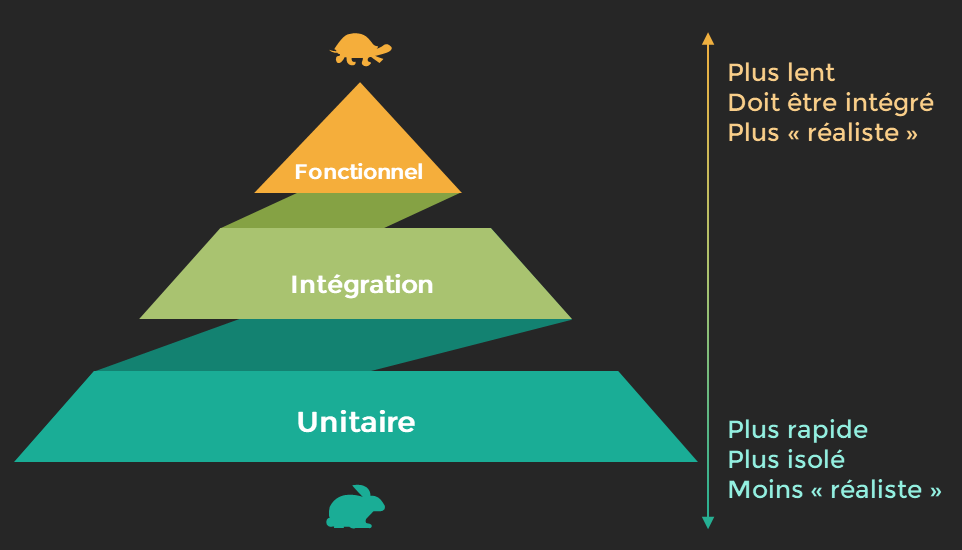
\includegraphics[width=7cm]{image/classic-test-pyramid}
        \end{columns}
        \bigbreak
        \footnotetext{OPENCLASSROOMS, Testez votre code Java pour réaliser des applications de qualité, \url{https://openclassrooms.com/fr/courses/6100311-testez-votre-code-java-pour-realiser-des-applications-de-qualite/6616481-decouvrez-les-tests-dintegration-et-les-tests-fonctionnels}}
        Mais d'autres valent le coup d'être découvertes\ldots

    \end{frame}

    \begin{frame}
        \transdissolve
        \frametitle{Testing}

        \begin{itemize}

            \item Un programme a pour entrée le standard input, et sorties les standard output et standard error, ce sont les standard streams
            \item Un programme se termine avec un code retour, le plus souvent un entier différent de 0 en cas de problème
            \item Les frameworks de tests retournent 3 statuts, OK, FAILED et ERROR
            \item Les OK si aucune erreur n'a lieu et FAILED en cas d'erreur d'assertion

        \end{itemize}

        \bigbreak

        \centering
        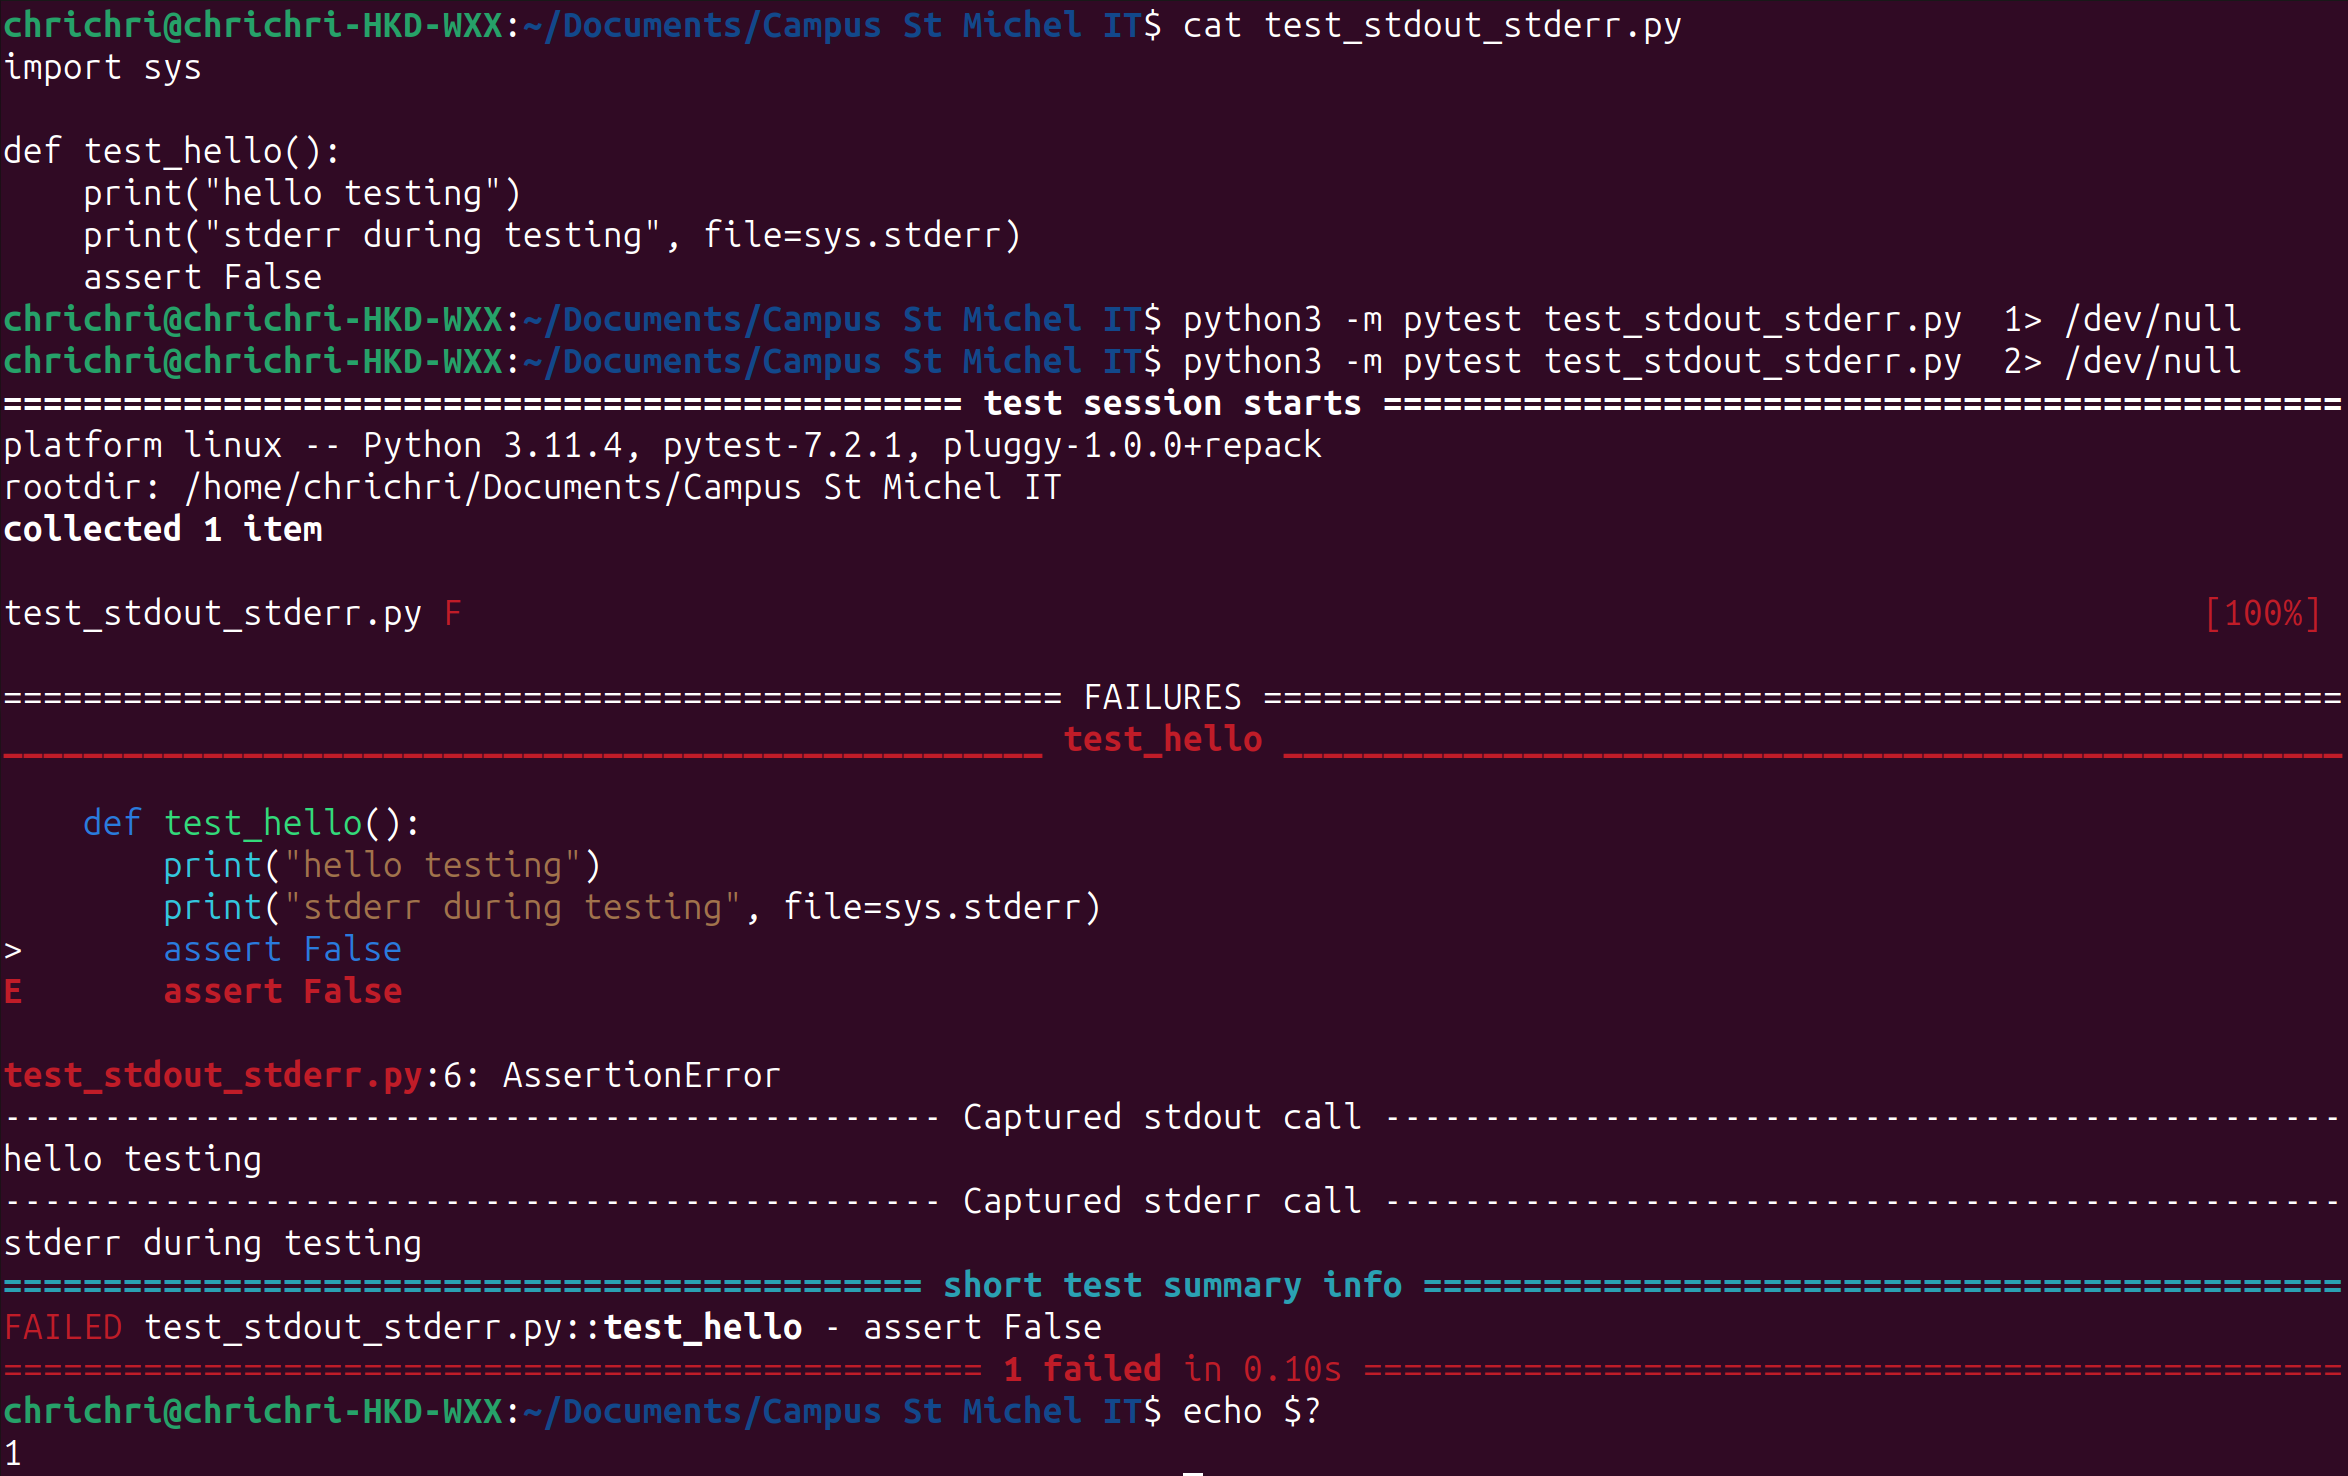
\includegraphics[width=7cm]{image/terminal-test-report}

    \end{frame}

    \begin{frame}
        \transdissolve
        \frametitle{Brief sur les outils de test logiciel}
        \begin{itemize}
            \item Les frameworks de test retournent 3 statuts, OK, FAILED et ERROR~.

            \item OK si aucune erreur n’a lieu et FAILED en cas d’erreur d’assertion, \lstinline{AssertionError} en Python et Java.

            \item Pas de standard universellement accepté mais un format domine, le XML JUnit.
            Un XML le définit par la grammaire \url{https://windyroad.com.au/dl/Open\%20Source/JUnit.xsd}.

            \item Vient de l’écosystème Java avec le package du même nom, JUnit, mais est présent dans la plupart des frameworks de test comme PHPUnit, Pytest.

            \item L’interopérabilité entre les outils est permise par cette XSD commune, mais pas plus de contrainte.
            Par exemple, l’interopérabilité entre les frameworks de test et les outils de CI/CD~.

            \item Certains outils, souvent des solutions propriétaires, rechignent toujours à exporter un JUnit contenant les résultats de test pour fermer leur environnement.

        \end{itemize}
    \end{frame}


    \begin{frame}[fragile]
        \frametitle{L'assertion error}
        \framesubtitle{En Python}
        \transdissolve
        L’instruction \lstinline{assert} vérifie une condition.
        Si la condition est vraie, cela ne fait rien et votre programme continue simplement à s’exécuter.
        Mais si la condition d’assertion est fausse, elle lève une exception \lstinline{AssertionError}.
        \begin{lstlisting}[language=Python]
assert 23 % 2 == 0, "Le restant de la division est différent de 0"
        \end{lstlisting}
        Étant toujours fausse, le programme crash.
        \begin{lstlisting}[language=sh]
chrichri@chrichri-HKD-WXX:~$ python3 -c 'assert 23 % 2 == 0, "Le restant de la division est différent de 0"'
Traceback (most recent call last):
  File "<string>", line 1, in <module>
AssertionError: Le restant de la division est différent de 0
        \end{lstlisting}
    \end{frame}

    \begin{frame}
        \frametitle{Pourquoi Pytest pour le testing}
        \transdissolve
        \textquote{pytest is a mature full-featured Python testing tool that helps you write better programs.\footnote{pytest: helps you write better programs , \url{https://docs.pytest.org}}}
        \begin{columns}
            \column{0.6\textwidth}
            Pytest est le framework de test en Python le plus utilisé selon les sondages de JetBrains\footnotemark.

            Seuls JUnit et Pytest sont pour tous usages, les autres sont orientés web.
            \column{0.4\textwidth}
            \centering
            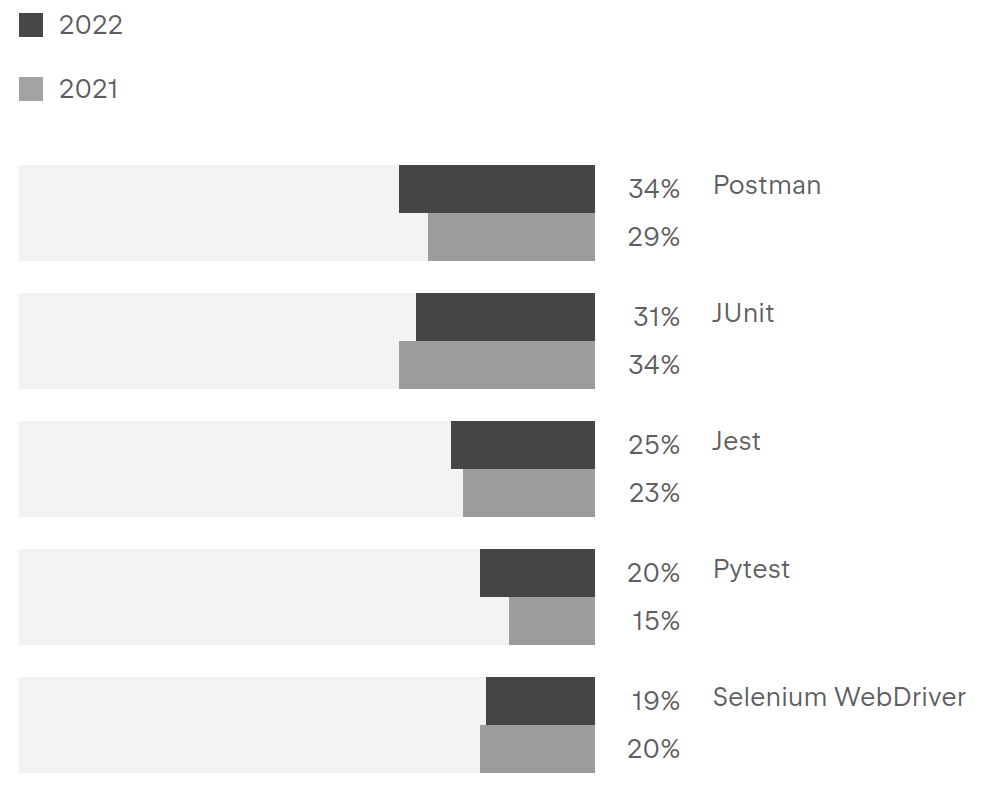
\includegraphics[width=5cm]{image/jetbrains-survey-testing-framework}
        \end{columns}
        \footnotetext{JetBrains, Which test frameworks , \url{https://www.jetbrains.com/lp/devecosystem-2022/testing/}}

    \end{frame}

    \begin{frame}[fragile]
        \frametitle{Pytest}
        \framesubtitle{Rédiger un test}
        \transdissolve
        \begin{itemize}
            \item Un module de test Pytest est un module Python préfixé par \lstinline{test_}.

            \item Toutes les méthodes préfixées par \lstinline{test_} sont exécutées par Pytest.
            Qu'elles soient dans une classe ou non.
            Les autres méthodes ne sont exécutées uniquement si les tests les appellent.
        \end{itemize}
        Ici par exemple, la précédente assertion est intégrée dans une méthode nommée \lstinline{test_divide} dans le module de test \lstinline{test_division.py}.
        \begin{lstlisting}[language=Python]
def test_divide():  # Un test Pytest est préfixé par test_
    assert 23 % 2 == 0, "Le restant de la division est différent de 0."
        \end{lstlisting}
    \end{frame}


    \begin{frame}[fragile]
        \frametitle{Pytest}
        \framesubtitle{Lancer les tests}
        \transdissolve
        Lancer avec la commande \lstinline{python -m pytest test_divison.py}, Pytest affiche le rapport de test.
        \begin{lstlisting}[language=sh]
...
def test_divide():  # Un test Pytest est préfixé par test_
>       assert 23 % 2 == 0, "Le restant de la division est différent de 0."
E       AssertionError: Le restant de la division est différent de 0.
E       assert (23 % 2) == 0

test_divison.py:2: AssertionError
...
        \end{lstlisting}

        De très utiles et nombreuses options peuvent compléter cette ligne de commande.
        Pour les découvrir, lancez \lstinline{python -m pytest --help} et \textquote{RTFM}.
    \end{frame}

    \begin{frame}[fragile]
        \frametitle{Pytest}
        \framesubtitle{Les tests paramétriques}
        \transdissolve
        Les tests paramétriques sont des tests qui prennent un ensemble de paramètres en entrées.

        Ils permettent de tester plusieurs cas avec un seul test.

        Le rapport génère un cas de test par paramètre.
        Il est donc plus détaillé et permet de trouvé
        les tests en échec plus facilement que si l'\lstinline {assert} était dans une boucle, ce qui ne donne qu'un statut OK ou Fail dans le rapport.
        \begin{lstlisting}[language=Python]
import pytest
...
@pytest.mark.parametrize("dividend", range(100))  # Paramétrage du test
def test_divide_from_0_to_99(dividend):  # Doit avoir un argument présent dans le paramétrage
    assert dividend % 2 == 0, "Le restant de la division est différent de 0."
        \end{lstlisting}
    \end{frame}

    \begin{frame}[fragile]
        \frametitle{Pytest}
        \framesubtitle{Les tests paramétriques}
        \transdissolve
        Génère 100 cas de tests.
        Met en évidence les dividendes dont le restant de la division par 2 est différent de 0, ici 1 par exemple.
        \begin{lstlisting}[language=sh]
collecting ... collected 100 items

test_divison.py::test_divide_from_0_to_99[0] PASSED                      [  1%]
test_divison.py::test_divide_from_0_to_99[1] FAILED                      [  2%]
test_divison.py:7 (test_divide_from_0_to_99[1])
1~!= 0

Expected~:0
Actual  ~:1
<Click to see difference>

dividend = 1

    @pytest.mark.parametrize("dividend", range(100))  # Paramétrage du test
    def test_divide_from_0_to_99(dividend):  # Doit avoir un argument présent dans le paramétrage
>       assert dividend % 2 == 0, "Le restant de la division est différent de 0."
E       AssertionError: Le restant de la division est différent de 0.
E       assert (1 % 2) == 0
        \end{lstlisting}
    \end{frame}

    \begin{frame}[fragile]
        \frametitle{Pytest}
        \framesubtitle{Plantage dans un test, quel statut?}
        \transdissolve
        Ce test crash avant l'assert.
        \begin{lstlisting}[language=Python]
def test_fail_or_error():  # Une erreur donne un fail ou error?
    dividende = 23 / 0
    assert dividende % 2 == 0, \
        "Le restant de la division est différent de 0."
        \end{lstlisting}
        Malgré l'absence d'\lstinline{assertionError}, le test est en échec et non en erreur.
        \begin{lstlisting}[language=sh]
test_divison.py::test_fail_or_error FAILED                               [100%]
test_divison.py:12 (test_fail_or_error)
def test_fail_or_error():  # Une erreur donne un fail ou error?
>       dividende = 23 / 0
E       ZeroDivisionError: division by zero

test_divison.py:14: ZeroDivisionError
        \end{lstlisting}

        \begin{dangercolorbox}
            Pour éviter les faux négatifs, un test doit tendre, tant que faire se peut, vers un \lstinline{assert}.
            Pour cela pensez à utiliser les fonctions \lstinline{parametrize} et \lstinline{fixture}.
        \end{dangercolorbox}
    \end{frame}

    \begin{frame}[fragile]
        \frametitle{Pytest}
        \framesubtitle{Les fixtures}
        \transdissolve
        Cf. \url{https://github.com/St-Michel-IT/testing/blob/main/test_customer_database.py}

        Un \lstinline{return} ou un \lstinline{yield} envoie l'objet au test dans l'état voulu.
        \begin{lstlisting}[language=Python]
def customer_without_table():
    """...
    """
    customer = Customer()  # Avant le test, c'est le setup
    yield customer  # Un yield évite de sortir de la fonction
    customer.con.close()  # Après le test, le teardown
        \end{lstlisting}
        Le test n'a qu'une seule ligne, qu'un \lstinline{assert} l'échec ne
        pourrait venir que de là.
        \begin{lstlisting}[language=Python]
def test_instantiation(customer_without_table):
    """...
    """
    assert isinstance(customer_without_table.con, Connection)
        \end{lstlisting}
        En cas de plantage dans la fixture, i.e., avant ou après le test, la sanction
        serait erreur et non échec.

        Le rapport reflétera fidèlement le test et sera exempt de faux négatif.
    \end{frame}

    \begin{frame}[fragile]
        \frametitle{Pytest}
        \framesubtitle{Les fixtures, le moyen du pattern A.A.A\footnote{Arrange-Act-Assert: A Pattern for Writing Good Tests, \url{https://automationpanda.com/2020/07/07/arrange-act-assert-a-pattern-for-writing-good-tests/}}}
        \transdissolve
        Le pattern du A.A.A, Arrange, Act, Assert, est facile à implémenter avec les fixtures.
        Arrange et Act sont isolé dans la fixture, Assert seul est dans le test.

        \begin{lstlisting}[language=Python]
def customer_without_table():
    """...
    """
    customer = Customer()  # Arrange et Act dans le setup avant yiel ou return
    yield customer
    customer.con.close()  # Pas de nom en A, ils l'ont oublié?
        \end{lstlisting}
        Le test tend vers un \lstinline{assert} quasi seul.
        \begin{lstlisting}[language=Python]
def test_instantiation(customer_without_table):
    """...
    """
    assert isinstance(customer_without_table.con, Connection) # Assert
        \end{lstlisting}
        Le B.D.D.~suit le pattern A.A.A sous un autre nom : Given-When-Then.
        Le langage Gherkin utilise les étapes Given-When-Then pour spécifier les comportements dans les scénarios.
    \end{frame}

    \begin{frame}
        \frametitle{Pytest}
        \framesubtitle{Exercice \execcounterdispinc{}, écrire un test avec une fixture}
        \transdissolve
        \textbf{Exercice~:} Écrivez votre premier test Pytest avec une fixture en respectant les exigences suivantes~:
        \begin{itemize}
            \item Le test doit utiliser une fixture avec setup et teardown.
            \item Le test doit respect le pattern A.A.A~.
        \end{itemize}
        \bigbreak
        Pour le setup et teardown, pensez à un fichier \emoji{winking-face}.
        \bigbreak
        Pour être évalué, créez un seul repo contenant tous les exercices de ce cours.
    \end{frame}

    \begin{frame}[fragile]
        \frametitle{Pytest}
        \framesubtitle{Le scope des fixtures}
        \transdissolve
        L'argument \lstinline{scope} du décorateur \lstinline{pytest.fixture} défini la durée de vie
        de la fixture.
        Il peut prendre 3 valeurs~:
        \begin{itemize}
            \item \lstinline{function}~: La valeur par défaut si on ne met rien.
            La fixture est exécutée à chaque fonction de test \lstinline{def test_...} qui l'appelle directement ou indirectement, donc les éventuels setup et teardown de cette dernière aussi.
            \item \lstinline{module}~: Une fois par module \lstinline{test_....py}.
            \item \lstinline{session}~: Une seule fois durant la session de test quel que soit le nombre de modules et de tests exécutés.
        \end{itemize}
        \begin{lstlisting}[language=Python]
@pytest.fixture(scope="function")  # Scope de la fixture, par default function
def customer_without_table():
    """Connection to in memory database using the Customer class"""
        \end{lstlisting}

        Pour tester une API en étant sûr le token n'est pas périmé, on peut utiliser le scope \lstinline{function} pour en avoir un nouveau à chaque appel.

        Si préparer les conditions initiales, le setup, prend du temps, on évitera si possible de le répéter à chaque test avec les scopes \lstinline{module}, \lstinline{session}.
    \end{frame}

    \begin{frame}
        \frametitle{Pytest}
        \framesubtitle{\lstinline{Le conftest.py}}
        \transdissolve
        Il n'a qu'une seule particularité, c'est d'être importé automatiquement par Pytest lorsqu'il est présent dans le dossier courant des tests.

        Il permet de factoriser les fixtures et les paramétrages de tests utilisés dans plusieurs modules de tests, car ces derniers seront automatiquement disponibles sans même un import dans le module.
        \begin{columns}
            \column{0.5\textwidth}
            \dirtree{%
                .1 ./.
                .2 {conftest.py}.
                .2 {\textcolor{flatgreen}{test\_no\_directory.py}}.
                .2 unit.
                .3 {\textcolor{flatgreen}{test\_integration.py}}.
                .2 functional.
                .3 {\textcolor{flatgreen}{test\_functional.py}}.
            }\column
            {0.5\textwidth}
            Pour tous ces tests, s'ils sont lancés depuis la racine avec la commande \lstinline{pytest}, le \lstinline{conftest.py} sera importé automatiquement.
        \end{columns}
        \bigbreak
        \begin{columns}
            \column{0.9\textwidth}
            PyCharm intègre par défaut Pytest comme lanceur de tests et fournit l'autocomplétion pour les fixtures du \lstinline{conftest.py}.
            \column{0.1\textwidth}
            \centering
            
\includegraphics[width=1cm]{image/logo-pycharm}
        \end{columns}
    \end{frame}

    \begin{frame}[fragile]
        \frametitle{Pytest}
        \framesubtitle{Le coverage}
        \transdissolve
        Pas de support natif du coverage par Pytest, il faut installer le plugin \lstinline{pytest-cov}\footnote{Welcome to pytest-cov’s documentation!, \url{https://pytest-cov.readthedocs.io/en/latest/}}.

        Pour appeler le plugin, il faut passer en argument le module à tester et le(s) test(s) de ce dernier.


        \begin{lstlisting}[language=sh]
pytest --cov=\textcolor{flatgreen}{customer_database} ./test_customer_database.py
...
rootdir: /home/chrichri/Documents/Campus-St-Michel-IT/testing
plugins: cov-4.1.0
collected 6 items

test_customer_database.py ......                                                                                                                                                                                                 [100%]

---------- coverage: platform linux, python 3.11.4-final-0 -----------
Name                   Stmts   Miss  Cover
------------------------------------------
customer_database.py       9      0   100%
------------------------------------------
TOTAL                      9      0   100%
        \end{lstlisting}

    \end{frame}

    \begin{frame}
        \frametitle{Pytest}
        \framesubtitle{Le coverage}
        \transdissolve
        \begin{columns}

            \column{0.5\textwidth}
            \centering
            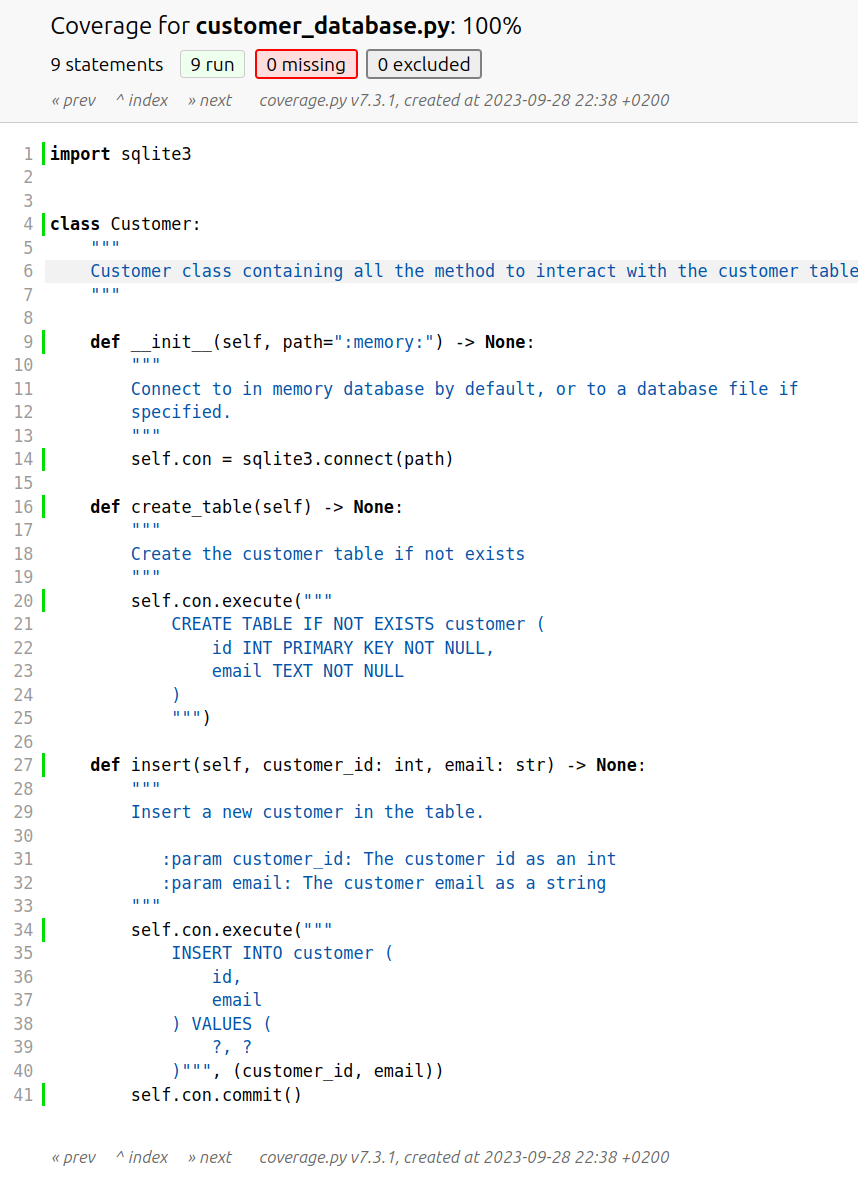
\includegraphics[width=5cm]{image/html-coverage}
            \column{0.5\textwidth}
            L'option \lstinline{--cov-report=html} permet de générer un rapport HTML plus détaillé qui met en lumière quelles parties du code sont couvertes par les tests et lesquelles ne le sont pas.
            \bigbreak
            \textbf{Exercice}~: Trouvez quel test du module \url{https://github.com/St-Michel-IT/testing/blob/main/test_customer_database.py} couvre quelle partie de ce code:
        \end{columns}

    \end{frame}

    \begin{frame}
        \frametitle{Pytest}
        \framesubtitle{Le secret de la réussite}
        \transdissolve
        \begin{columns}
            \column{0.7\textwidth}
            Pytest est un framework complet voir complexe.

            Mais quasi toutes les fonctionnalités auxquelles on peut penser sont déjà implémentées et décrites une documentation de qualité.

            Comme avec toutes les grosses libraries, il faut avoir confiance en leur design et chercher dedans avant de réinventer la roue.

            La liste des fonctionnalités est trop longue, nous venons juste d'en découvrir les principales.
            \bigbreak
            Donc une fois encore, comme pour toutes les bonnes libraires à connaître, le secret est \textquote{\textbf{\Large{RTFM}}}~!
            \column{0.3\textwidth}
            \centering
            
\includegraphics[width=3cm]{image/girl-rtfm}
        \end{columns}
    \end{frame}

    \begin{frame}
        \frametitle{Pytest}
        \framesubtitle{Travaux dirigés sur les tests unitaires}
        \transdissolve
        \textbf{Exercice \execcounterdispinc{}}~: Toujours à partir de la librairie du repo \url{https://github.com/St-Michel-IT/testing/}, où le module \lstinline{customer_database.py} est testé par \lstinline{test_customer_database.py}.
        Ajoutez une méthode qui modifie les données d'un client et les tests qui vont avec.
        \bigbreak
        \textbf{Exercice \execcounterdispinc{}}~: Toujours dans le même repo, le module \lstinline{witness_number.py} est un début implémentation d'une généralisation du petit théorème de Fermat expliquée sur la chaîne Youtube Numberphile par Matt Parker\footnote{Numberphile, Witness Numbers (and the truthful 1,662,803), \url{https://www.youtube.com/watch?v=_MscGSN5J6o}}.
        Cette librairie n'est pas déjà libre sur le web.
        Finissons son développement, en implémentant \textbf{toutes les fonctionnalités de la vidéo} de M. Parker avec des standards de qualité élevés grâce à nos connaissances en testing.
    \end{frame}


    \section{Le mutation testing}\label{sec:mutation-testing}

    \begin{frame}[fragile]
        \frametitle{Mutation testing}
        \framesubtitle{Vérifier la qualité des tests unitaires}
        \transdissolve
        Imaginez un test sans assert, il ne fait qu'exécuter le code.
        Tout le code est couvert, mais le test ne sert à rien.
        % Python listing
        \begin{lstlisting}[language=Python]
def test_fibonacci():
    fibonacci()
        \end{lstlisting}
        \bigbreak
        Quel est le coverage~?
        \pause
        Il peut être de 100\%.
        Encore une fois cette métrique n'est pas suffisante pour juger de la qualité des tests.
        \bigbreak
        Le mutation est une étape qui intervient \textbf{quand tous les tests unitaires passent uniquement}.
        Cette étape consiste à modifier le code source pour voir si les tests échouent.
        C'est un raisonnement par l'absurde.
        Ils doivent en effet échouer pour prouver qu'ils testent le comportement du code et ne font pas que l'exécuter.
    \end{frame}

    \begin{frame}
        \frametitle{Mutation testing}
        \framesubtitle{Fonctionnement des librairies comme \lstinline{mutmut}\footnote{mutmut - python mutation tester, \url{https://mutmut.readthedocs.io/en/latest/}}}
        \transdissolve
        La librairie de mutation essaie de modifier le code avec par exemple les règles suivantes~:
        \begin{itemize}
            \item Changer les opérateurs mathématiques, comme \lstinline{+} en \lstinline{-}, \lstinline{>} en \lstinline{>=}
            \item Changer les opérateurs logiques : \lstinline{and} en \lstinline{or} et inversement
            \item Intervertir les mots-clés, comme \lstinline{True}/\lstinline{False}, \lstinline{in}/\lstinline{not} in
            \item Intervertir \lstinline{copy} et \lstinline{deepcopy}
            \item Remplacer \lstinline{""} par \lstinline{None}
            \item Changer les valeurs numériques en ajoutant \lstinline{1}
            \item Changer les valeurs des chaînes de caractères en ajoutant \lstinline{"xx"}
            \item Changer les noms des arguments des fonctions en ajoutant \lstinline{"xx"}
        \end{itemize}
    \end{frame}


    \begin{frame}[fragile]
        \frametitle{Mutation testing}
        \framesubtitle{Example avec \lstinline{mutmut}}
        \transdissolve
        Dans le dossier \lstinline{mutmut_fib} il y a 11 tests unitaires qui passent~:
        \begin{lstlisting}[language=bash,basicstyle=\ttfamily\tiny]
$ python -m pytest tests/test_fib.py
================================================================ test session starts ======
platform linux -- Python 3.11.6, pytest-7.4.2, pluggy-1.3.0
rootdir: /home/chrichri/Documents/Campus-St-Michel-IT/testing/mutmut_fib
plugins: cov-4.1.0
collected 11 items

tests/test_fib.py ...........                                                                                                                  [100%]

================================================================= 11 passed in 0.04s ======
        \end{lstlisting}
        Quand un mutant est détecter par les tests, il est \textquote{tué}.
        Les \textquote{survivants} indiquent que les tests ne sont pas suffisants.
        Ici \lstinline{mutmut} créé 5 mutants, donc 5 versions différentes de la fonction \lstinline{mutmut_fib.src.fib.fibonacci}, tous tués.
        \begin{lstlisting}[language=bash,basicstyle=\ttfamily\tiny]
venv) chrichri@chrichri-HKD-WXX:~/Documents/Campus-St-Michel-IT/testing/mutmut$ mutmut show 3
--- src/fib.py
+++ src/fib.py
@@ -1,6 +1,6 @@
 def fibonacci(n: int) -> int:
     """Get the n-th Fibonacci number"""
-    a, b = 0, 1
+    a, b = None
     for _ in range(n-1):
         a, b = b, a + b
     return a
        \end{lstlisting}
    \end{frame}

    \begin{frame}
        \frametitle{Mutation testing}
        \framesubtitle{Example avec \lstinline{mutmut}}
        \transdissolve
        \centering
        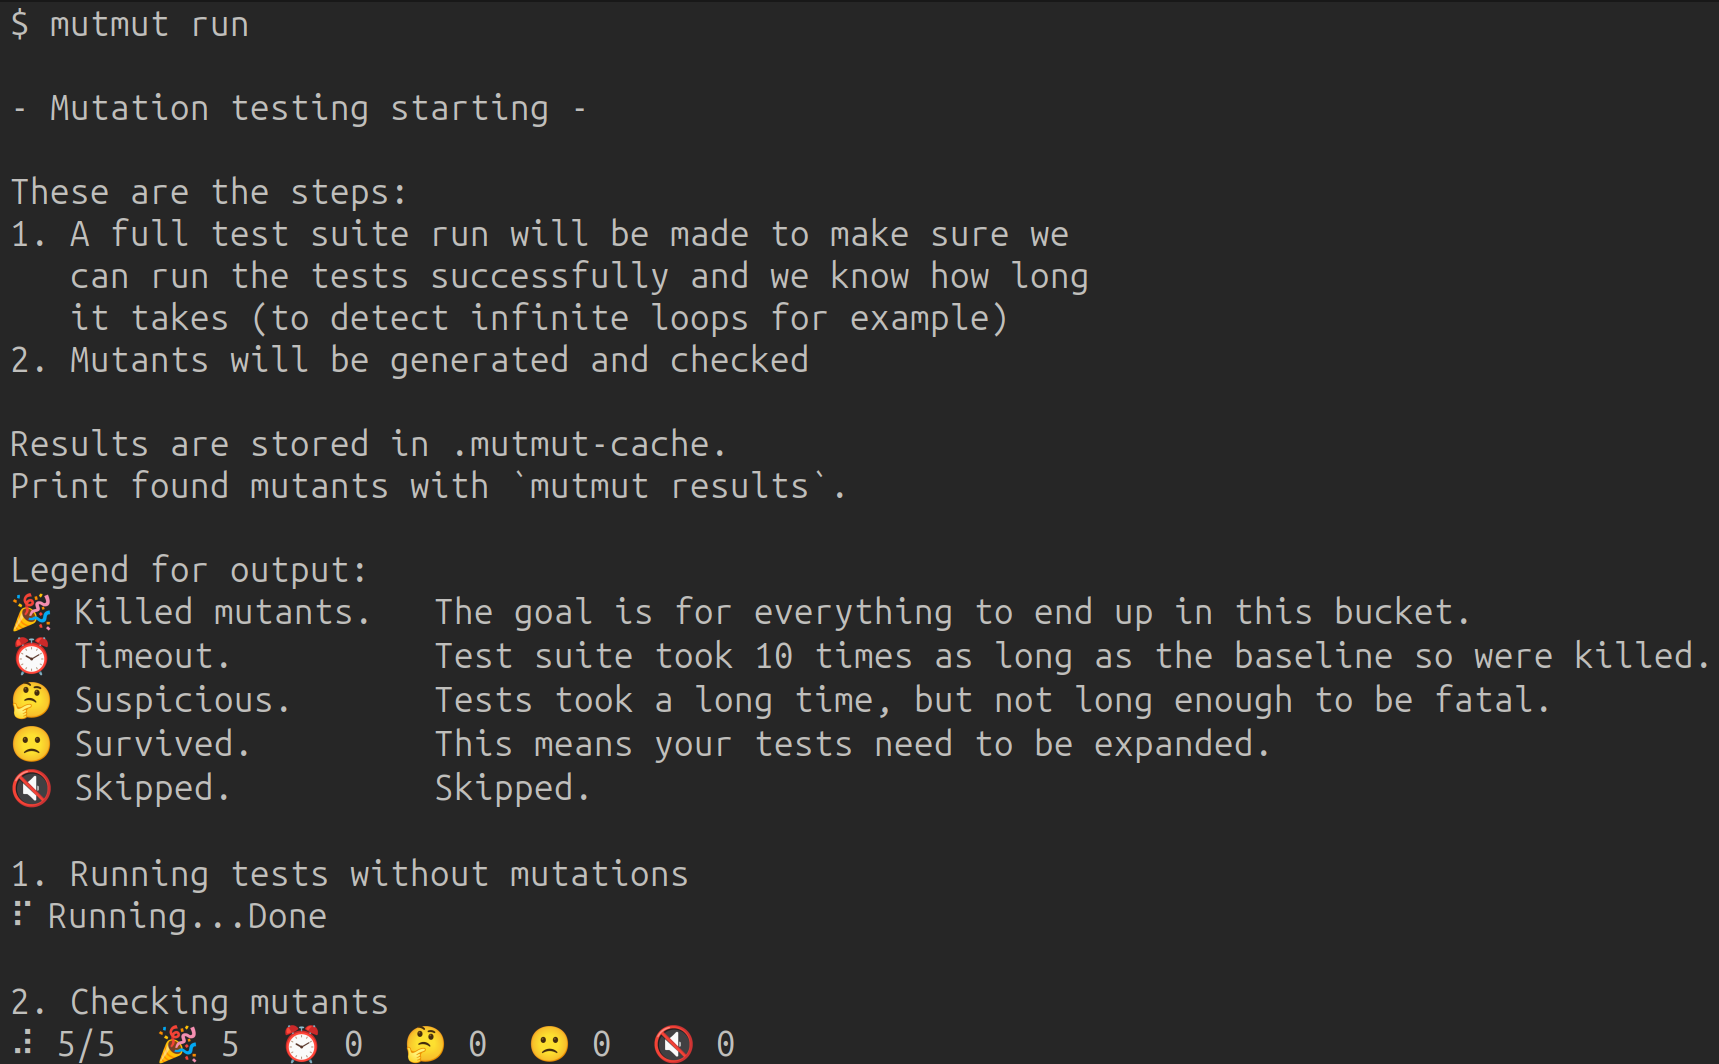
\includegraphics[width=11cm]{image/mutmut-result}
    \end{frame}

    \begin{frame}
        \frametitle{Mutation testing}
        \framesubtitle{Conclusion}
        \transdissolve
        Un rapport de test unitaire devrait contenir~:
        \begin{itemize}
            \item Les rapport de test avec les résultats des tests unitaires
            \item Le rapport de test coverage
            \item Le rapport de mutation testing
        \end{itemize}
        \centering
        
\includegraphics[width=7cm]{image/mutant}
    \end{frame}


    \section{Le BDD}\label{sec:le-bdd}
    \begin{frame}
        \frametitle{Tests avec langage naturel}
        \framesubtitle{A.K.A le BDD}
        \transdissolve

        \begin{dangercolorbox}
            Les slides qui suivent sont truffés de biais négatifs sur le BDD suite à de mauvaises expériences \emoji{grinning-face-with-sweat}.

        \end{dangercolorbox}
        Le BDD est le sigle de Behavior-Driven Development.
        \begin{columns}
            \column{0.7\textwidth}
            Vous remarquerez qu'il n'y ici aucune mention liée au testing?

            Alors pourquoi est-il régulièrement associé au testing~?
            \column{0.3\textwidth}
            \centering
            
\includegraphics[width=3cm]{image/funny-drawing-of-a-cucumber}
        \end{columns}
        Parce que le BDD est un outil de communication entre les développeurs et les métiers qui permet à ceux qui spécifient le produit de le décrire par rapport au comportement (behavior) attendu.
        Le tout dans une syntaxe proche du langage naturel.
        Ce langage peut être utilisé pour générer des tests.
        On pourrait presque finir par croire que le métier peut écrire les tests.
    \end{frame}

    \begin{frame}
        \frametitle{Tests avec langage naturel}
        \framesubtitle{Cucumber ne serait même pas un outil de test}
        \transdissolve
        Dans cette \href{https://news.ycombinator.com/item?id=10194242}{discussion sur Ycombinator}, le créateur de Cucumber affirme plusieurs choses intéressantes dont~:
        \begin{itemize}
            \item \textquote{The biggest problem with Cucumber is that most people trying it out don't understand what it is.}
            \item \textquote{Cucumber is not a tool for testing software.}
            \item \textquote{Cucumber is a tool that facilitates collaboration and software design (especially domain-driven design).}
            \item \textquote{The purpose of Cucumber is to bridge the communication gap between business and IT by providing a small set of essential scenarios to illustrate core behaviour of unwritten software.}
        \end{itemize}
        Mais comme c'est au programme et que ça ne choque plus grand monde on va s'en servir d'outil de test quand même. \emoji{smiling-face-with-halo}
    \end{frame}

    \begin{frame}[fragile]
        \frametitle{Spécifier avec le BDD}
        \framesubtitle{Exemple de Cucumber, le plus répandu}
        \transdissolve
        Développé en début des années 2000 par Daniel Terhorst-North, il fait entre autre le constat que~: \textquote{Behaviour} is a more useful word than \textquote{test}\footnote{Daniel Terhorst-North, Introducing BDD, \url{https://dannorth.net/introducing-bdd/}}.
        \bigbreak
        Il utilise les mots clés \textquote{Given}, \textquote{When} et \textquote{Then} pour décrire le comportement attendu du produit en développement dans un scénario.
        \begin{lstlisting}
Given some initial context (the givens),
When an event occurs,
Then ensure some outcomes.
        \end{lstlisting}

        Par exemple~:
        \begin{lstlisting}
Given I just openned a new private window in my browser
When I browse the https://in-france.fr website
Then I wan to descover the french economy by activity
And by region.
        \end{lstlisting}

        On comprend facilement que ce sont des critères d'acceptation haut niveau.
        Les tests liés seront donc des tests d'acceptation/fonctionnels.
    \end{frame}

    \begin{frame}
        \frametitle{Spécifier avec le BDD}
        \framesubtitle{Exemple de Cucumber\footnote{Given-When-Then pattern in unit tests, \url{https://www.j-labs.pl/blog-technologiczny/given-when-then-pattern-in-unit-tests/}}}
        \transdissolve
        \begin{columns}
            \column{0.5\textwidth}
            \centering
            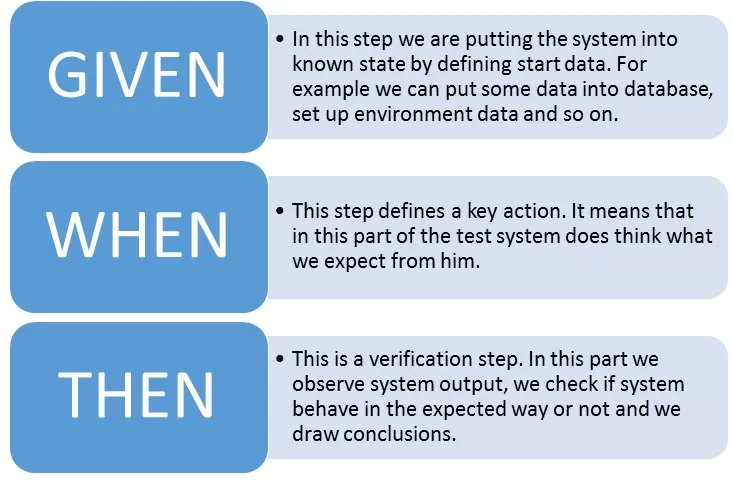
\includegraphics[width=6cm]{image/given-when-then}
            \column{0.5\textwidth}
            \centering
            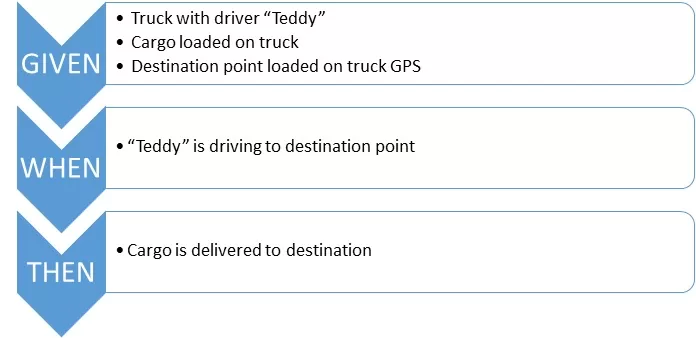
\includegraphics[width=6cm]{image/given-when-then-exemple}
        \end{columns}
        \textquote{And} peut être utilisé pour ajouter des conditions supplémentaires aux 3 mots clés précédents\footnote{Getting Started with BDD, \url{https://cucumber.io/blog/bdd/getting-started-with-bdd-part-1/}}.
    \end{frame}

    \begin{frame}[fragile]
        \frametitle{Spécifier avec le BDD}
        \framesubtitle{Exemple de Cucumber, le plus répandu}
        \transdissolve
        Les données d'un test paramétrique sont définies dans un tableau\footnote{Given/When/Then And Example Tables Using the Robot Framework, \url{https://www-codecentric-de.translate.goog/wissens-hub/blog/givenwhenthen-and-example-tables-using-the-robot-framework?_x_tr_sl=en&_x_tr_tl=fr&_x_tr_hl=fr&_x_tr_pto=sc&_x_tr_hist=true}}.
        \begin{lstlisting}[basicstyle=\ttfamily\tiny]
Example
    [Arguments]  ${periodClosed}  ${periodOpenAndModified}  ${importDay}  ${oldManagerValidUntil}  ${newManagerValidFrom}

    Given initialized criteria for bonus commercial
    And a branch B with branch manager M_OLD and employee E1
    And evaluation for E1 for period ${periodClosed} which is closed
    And evaluation for E1 for period ${periodOpenAndModified} which is open and modified

    When M_NEW becomes new manager of branch B
    And import service is called on ${importDay}
    Then the new branch manager of branch B is M_NEW valid from ${newManagerValidFrom}
    And branch manager M_OLD manages employee E until ${oldManagerValidUntil}
    And branch manager M_NEW manages employee E from ${newManagerValidFrom}
    And Evaluations for E1 still have the same content

| *Test Case* | | *Closed Period*        | *Open Period*          | *Run Import On* | *Old Manager Stops* | *New Manager Starts* |
| 1 | Example   | 1.11.2009 - 30.11.2009 | 1.12.2009 - 31.12.2009 | 11.11.2009      | 30.11.2009          |  1.12.2009
| 2 | Example   | 1.11.2009 - 30.11.2009 | 1.12.2009 - 31.12.2009 |  1.11.2009      | 31.10.2009          |  1.11.2009
        \end{lstlisting}
    \end{frame}

    \begin{frame}[fragile]
        \frametitle{BDD qui a-t-il derrière ce langage~?}
        \framesubtitle{Quelques exemples en Python et Java}
        \transdissolve
        Avec Behave en Python\footnote{Tutorial, \url{https://behave.readthedocs.io/en/latest/tutorial/\#features}}~:
        \begin{lstlisting}
features/
features/everything.feature
features/steps/
features/steps/steps.py
        \end{lstlisting}
        Derrière une phrase~:
        \begin{lstlisting}
from behave import then

@then('the result page will include "{text}"')
def step_impl(context, text):
    if text not in context.response:
        fail('%r not in %r' % (text, context.response))
        \end{lstlisting}
        Avec Cucumber en Java\footnote{Cucumber Java, \url{https://cucumber.io/docs/guides/10-minute-tutorial/}}~:
        \begin{lstlisting}
@When("the stock is traded at $price")
public void theStockIsTradedAt(double price) {
    stock.tradeAt(price);
}
        \end{lstlisting}
        \bigbreak
        C'est une illusion de simplicité, derrière le langage naturel, il y a quasiment la même algorithmique.
    \end{frame}

    \begin{frame}
        \frametitle{Exercice \execcounterdispinc{} de BDD}
        \framesubtitle{Exemple de Cucumber, le plus répandu}
        \transdissolve
        \textbf{Exercice~:} En utilisant un maximum du code de l'exercice précédent sur les nombres témoins, réécrivez l'équivalent des tests pytest ou autre en scénarios Behave.
    \end{frame}


    \section{Le TDD}\label{sec:le-tdd}

    \begin{frame}
        \transdissolve
        \frametitle{Le TDD}
        \framesubtitle{Test Driven Development}
        Vouloir aller plus vite sans faire de test semble être une mauvaise idée.

        Ce qui pratiquent le TDD vont plus vite dès le début d'un projet\footnote{\label{cleanarchitecture}Clean architecture, Robert C. Martin}~!

        Entre autre, les tests unitaires font réduire la taille des classes, functions et des méthodes, ce qui améliore architecture.
        \begin{columns}
            \column{0.3\textwidth}
            \textquote{The only way to go fast, is to go well\cref{cleanarchitecture}.}
            \column{0.7\textwidth}
            \centering
            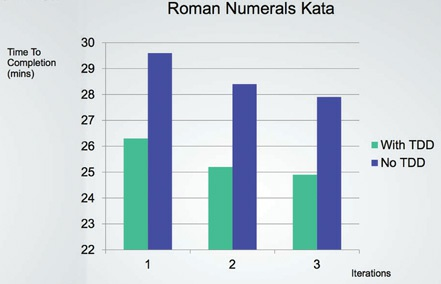
\includegraphics[width=7cm]{image/tdd-vs-no-tdd}
        \end{columns}
    \end{frame}

    \begin{frame}
        \transdissolve
        \frametitle{Le TDD}
        \framesubtitle{Quel type(s) de test~?}
        Tous les types de tests possibles sont à écrire dès que possible avant même de commencer à coder.
        Les tests unitaires sont en général les plus simples à écrire et les plus rapides à exécuter.
        \bigbreak
        Les éléments centraux, les règles de gestions, les \textquote{business rules} doivent être testables sans les éléments périphériques\cref{cleanarchitecture}~:
        \bigbreak
        \centering
        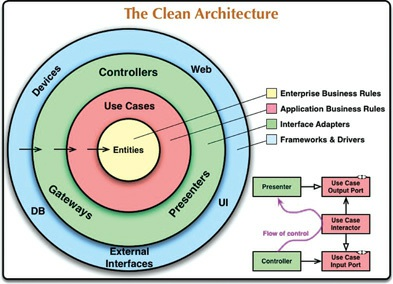
\includegraphics[width=6cm]{image/the-clean-architecture}
    \end{frame}

    \begin{frame}
        \transdissolve
        \frametitle{Le TDD}
        \framesubtitle{Quel types de test~?}
        Edsger Dijkstra~: \textquote{Testing shows the presence, not the absence of bugs.}
        \bigbreak
        \begin{columns}
            \column{0.5\textwidth}
            Autrement dit, l'univers des tests est infini, on n'a jamais la certitude de suffisamment tester.
            \bigbreak
            Même le coverage est une mauvaise mesure.
            \column{0.5\textwidth}
            \centering
            
\includegraphics[width=5cm]{image/monk-looking-the-deepness-of-the-stars-in-the-night-sky}
        \end{columns}
    \end{frame}

    \begin{frame}
        \transdissolve
        \frametitle{Le TDD}
        \framesubtitle{Exercices \execcounterdispinc{}}
        De nombreux exercices de TDD sont disponibles sur le web comme par sur GitHub, \url{https://github.com/gabbloquet/entrainement-au-tdd}.
        \bigbreak
        En 30 minutes, sans assistant du type ChatGPT, réaliser l'un des plus classique d'entre eux, le \textquote{FizzBuzz}, \url{https://github.com/gabbloquet/entrainement-au-tdd/tree/master/src/main/java/io/github/gabbloquet/tddtraining/FizzBuzz}~.
        Respecter l'esprit du TDD qui veut que l'on écrive les tests avant le code~:
        \begin{enumerate}
            \item Écrire un test par requirement.
            \item Écrire l'algorithme.
            \item Refactoriser.
            \item Revenir à l'étape 2 jusqu'à ce que tous les test passent.
        \end{enumerate}
    \end{frame}


    \section{Tests assistés par l'IA}\label{sec:tests-assistes-par-ia}

    \begin{frame}[fragile]
        \transdissolve
        \frametitle{Tests assisté par l'IA}
        \framesubtitle{Test de GitHub Copilot le 30 mai 2024}
        Based on your request, here are some unit tests for the \lstinline{Customer} class in the \lstinline{customer_database.py} module.
        These tests cover the happy path and some edge cases for the \lstinline{create_table} and \lstinline{insert} methods.
        The test names are self-explanatory and do not start with \textquote{test}.
        The tests are written using the \lstinline{unittest} module, which is a built-in module in Python for writing tests.
        \begin{lstlisting}[language=Python]
import sqlite3
import unittest
from unittest.mock import Mock

from customer_database import Customer

class CustomerDatabaseTests(unittest.TestCase):
    def setUp(self):
        ...
    def creating_customer_table(self):
        self.customer.create_table()
        ...
        \end{lstlisting}
        These tests use the \lstinline{unittest.mock} module to mock the \lstinline{sqlite3.connect} function, allowing us to test \ldots
    \end{frame}

    \begin{frame}[fragile]
        \transdissolve
        \frametitle{Tests assisté par l'IA}
        \framesubtitle{Test de GitHub Copilot le 30 mai 2024}
        \begin{lstlisting}
(venv) chrichri@chrichri-HKD-WXX:~/Documents/Campus-St-Michel-IT/testing$ python -m unittest test_customer_database_with_copilot.py

----------------------------------------------------------------------
Ran 0 tests in 0.000s

OK
        \end{lstlisting}
        \textquote{All tests should start with def test\_ no ? To be compliant with unittest?}
        \bigbreak
        Yes, you're correct.
        In Python's \lstinline{unittest} module, test methods should start with \lstinline{test_}.
        This is how the test runner identifies which methods represent tests.
        Here's how you can modify the test methods in your \lstinline{CustomerDatabaseTests} class:
    \end{frame}

    \begin{frame}[fragile]
        \transdissolve
        \frametitle{Tests assisté par l'IA}
        \framesubtitle{Test de GitHub Copilot le 30 mai 2024}
        \begin{lstlisting}[language=Python]
class CustomerDatabaseTests(unittest.TestCase):
    def setUp(self):
        ...
    def test_creating_customer_table(self):
        ...
        \end{lstlisting}
        Now, each test method starts with \lstinline{test_}, making them compliant with \lstinline{unittest}.
        \begin{lstlisting}
Error
Traceback (most recent call last):
  File "/home/chrichri/Documents/Campus-St-Michel-IT/testing/ble_to_rpc_client.py", line 9, in setUp
    self.customer = Customer(self.mock_db)
                    ^^^^^^^^^^^^^^^^^^^^^^
  File "/home/chrichri/Documents/Campus-St-Michel-IT/testing/customer_database.py", line 14, in __init__
    self.con = sqlite3.connect(path)
               ^^^^^^^^^^^^^^^^^^^^^
TypeError: expected str, bytes or os.PathLike object, not Mock
        \end{lstlisting}
        En conclusion, on a encore besoin de l'humain...
    \end{frame}

    \begin{frame}[fragile]
        \transdissolve
        \frametitle{Tests assisté par l'IA}
        \framesubtitle{Cover Agent}
        Un framework open source qui utilise la puissance de l'IA pour générer des tests unitaires.
        Compatible avec la plupart des LLMs grâce à \href{https://www.litellm.ai/}{LiteLLM handles loadbalancing, fallbacks and spend tracking across 100+ LLMs. All in the OpenAI format}. Voir sa page GitHub\footnote{Cover Agent, \url{https://github.com/Codium-ai/cover-agent}}.
        \bigbreak
        Exercice \execcounterdispinc{}~: Tester le code \url{https://github.com/St-Michel-IT/testing/blob/main/test_customer_database.py} avec Cover Agent.
    \end{frame}


    \section{Les tests d’intégration}\label{sec:les-tests-d-integration}

    \begin{frame}
        \transdissolve
        \frametitle{Les tests d'intégration}
        \framesubtitle{définition}
        Les tests d’intégrations sont des tests effectués entre les composants afin de s’assurer du fonctionnement des interactions et de l’interface entre les différents composants.
        Ces tests sont également gérés, en général, par des développeurs\footnote{Les niveaux de test, \url{https://latavernedutesteur.fr/2017/11/03/les-niveaux-de-test/}}.
        \begin{columns}
            \column{0.5\textwidth}
            C'est aussi la définition de l'ISTQB\footnotemark~.
            \column{0.5\textwidth}
            \centering
            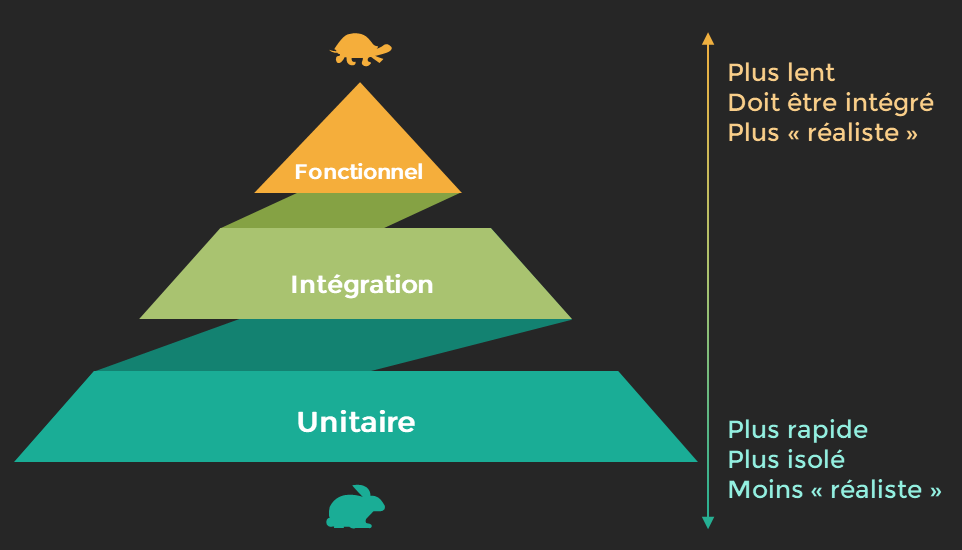
\includegraphics[width=5cm]{image/classic-test-pyramid}
        \end{columns}
        \footnotetext{Glossaire CFTL/ISTQB des termes utilisés en tests de logiciels, \url{https://www.cftl.fr/wp-content/uploads/2018/10/Glossaire-des-tests-logiciels-v3_2F-ISTQB-CFTL-1.pdf}}
    \end{frame}

    \begin{frame}
        \transdissolve
        \frametitle{Les tests d'intégration}
        \framesubtitle{définition}
        Autrement dit, les tests unitaires on testés chaque composant, ceux d'interactions testent les interactions entre les composants.
        \bigbreak
        \centering
        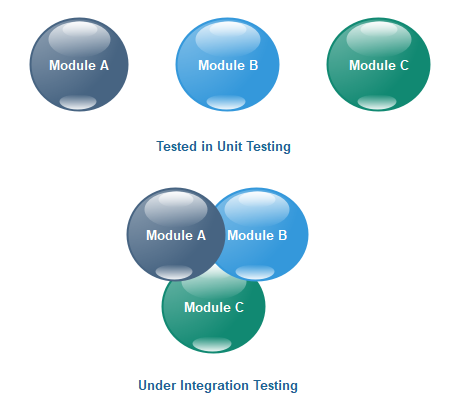
\includegraphics[width=7cm]{image/integration-testing-vs-unit-testing}
    \end{frame}

    \begin{frame}
        \transdissolve
        \frametitle{Les tests d'intégration}
        \framesubtitle{les différentes approches, les top-down, bottom-up et mixte\footnote{\label{unice-ti} Tests d’intégration, \url{https://mbf-iut.i3s.unice.fr/lib/exe/fetch.php?media=undefined:7-testintegration-2016.pdf}}}
        La top-down consiste à tester les composants les plus hauts de la hiérarchie en premier.
        \break
        La bottom-up consiste à tester les composants les plus bas de la hiérarchie en premier.
        \begin{columns}
            \column{0.33\textwidth}
            \centering
            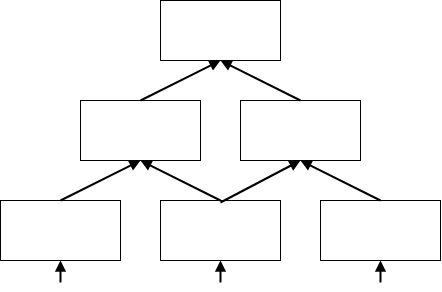
\includegraphics[width=4cm]{image/ti-bottom-up.drawio} \\ Bottom-up \\
            \column{0.33\textwidth}
            \centering
            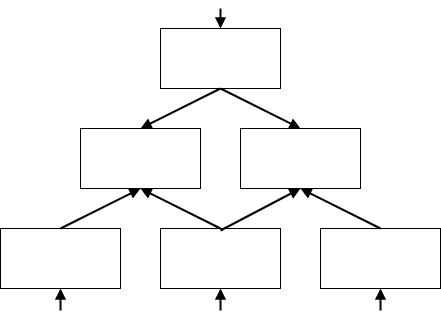
\includegraphics[width=4cm]{image/ti-mixte.drawio} \\ Mixte \\
            \column{0.33\textwidth}
            \centering
            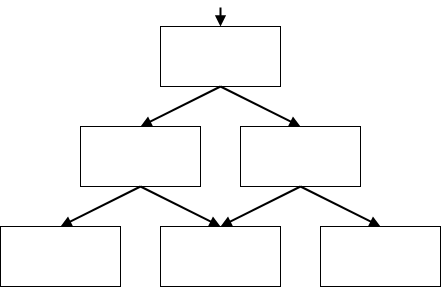
\includegraphics[width=4cm]{image/ti-top-down.drawio} \\ Top-down \\
        \end{columns}
    \end{frame}

    \begin{frame}
        \transdissolve
        \frametitle{Les tests d'intégration}
        \framesubtitle{Bonnes pratiques}
        \begin{itemize}
            \item Ne pas tester la logique métier, c'est le rôle des tests unitaires.
            \item Ne pas les mélanger à d'autres tests, unitaire ou autre.
            \item Ils testent les interfaces.
            \item Ils sont généralement plus longs à jouer, il est donc conseillé de bien séparer les suites de test pour pouvoir lancer un sous-ensemble précis.
        \end{itemize}
    \end{frame}

    \begin{frame}
        \transdissolve
        \frametitle{Les tests d'intégration}
        \framesubtitle{Exemple}

        Les 15 lignes de code \url{https://github.com/St-Michel-IT/testing/blob/main/ble_to_rpc.py} permettent de récupérer des données du Bluetooth Low Energy (BLE) et les distribuer \textquote{over} HTTP au format JSON RPC~.
        \bigbreak
        C'est donc l'intégration de 3 librairies~:
        \begin{itemize}
            \item \href{https://bleak.readthedocs.io/en/latest/index.html}{\lstinline{bleak}} pour le BLE~.
            \item \href{https://werkzeug.palletsprojects.com/en/3.0.x/}{\lstinline{Werkzeug}} pour le serveur HTTP~.
            \item \href{https://github.com/pavlov99/json-rpc}{\lstinline{json-rpc}} pour le format des données.
        \end{itemize}
        \bigbreak
        Le tester est donc bien un test d'intégration de ces librairies.
    \end{frame}

    \begin{frame}
        \transdissolve
        \frametitle{Les tests d'intégration}
        \framesubtitle{Exercice \execcounterdispinc{}}
        \begin{columns}
            \column{0.7\textwidth}
            Proposer et rédiger des tests d'intégration pour le code \url{https://github.com/St-Michel-IT/testing/blob/main/ble_to_rpc.py}.
            Dans la techno de votre choix.
            \bigbreak
            Tester les 3 protocoles intégrés.
            \bigbreak
            Ajouter la fonction de connection BLE à un appareil définie par son adresse et lire la caractéristique \textquote{GATT} \lstinline{2A24}.
            Rédiger également les tests correspondant.
            \column{0.3\textwidth}
            \centering
            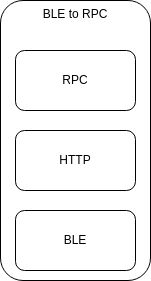
\includegraphics[width=3cm]{image/ble-2-rpc-stack.drawio}
        \end{columns}
    \end{frame}

    \begin{frame}
        \transdissolve
        \frametitle{Les tests d'intégration}
        \framesubtitle{Exercice \execcounterdispinc{}}
        \begin{columns}
            \column{0.7\textwidth}
            Ils peuvent aussi être utilisés en embarqué, IOT, etc.
            \bigbreak
            En lisant la documentation Arduino  \url{https://github.com/St-Michel-IT/testing/blob/main/doc/Arduino\%C2\%AE\%20UNO\%20R3\%20Datasheet.pdf}, ajouter des tests d'intégration au module de test \url{https://github.com/St-Michel-IT/testing/blob/main/test_arduino.py}.
            \column{0.3\textwidth}
            \centering
            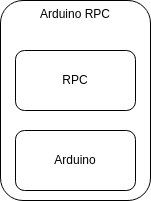
\includegraphics[width=3cm]{image/arduino-rpc-stack.drawio}
        \end{columns}
    \end{frame}


    \section{Intégration Continue}\label{sec:ci}

    \subsection{Généralité}\label{subsec:ci-general}
    \begin{frame}
        \frametitle{Intégration continue A.K.A. CI}
        \framesubtitle{Les defintions du CI/CD}
        \transdissolve
        CI/CD est l'acronyme de \textquote{Continuous Integration/Continuous Delivery} ou \textquote{Continuous Deployment}.
        \bigbreak
        \textquote{le but ultime du processus CI/CD qui consiste à supprimer l’intervention humaine pour gagner en temps et en efficacité. Le code est compilé et testé sur l’ordinateur grâce à ce que l’on appelle un build automatisé. S’il n’y a pas de bug le tout est mis en production automatiquement. Cette approche permet aux développeurs de se concentrer sur la conception et le développement et sur les fonctionnalités de l’application.}\footnote{Qu'est-ce que l'approche CI/CD - Qu’est-ce que le processus CI/CD ?, \url{https://www.oracle.com/fr/cloud/definition-approche-ci-cd/}}
        \bigbreak
        \centering
        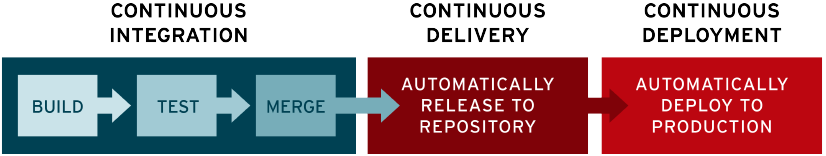
\includegraphics[width=7cm]{image/ci-cd-flow.png}
    \end{frame}

    \begin{frame}
        \frametitle{Intégration continue A.K.A. CI}
        \framesubtitle{Les defintions du CI/CD}
        \transdissolve
        Plusieurs remarques~:
        \begin{itemize}
            \item Une des avancées est l'automatisation de multiples taches.
            \item Le mot intégration fait penser qu'on a plusieurs systèmes, logiciels, développeurs, équipes, etc.
            \item L'\textquote{ordinateur} n'est pas définit, on verra qu'il peut être celui du développeur ou un serveur distant voir un ordinateur inconnu.
            \item \textquote{S’il n’y a pas de bug le tout est mis en production automatiquement.} vous y croyez?
            \item Le but est toujours le même, éliminer un maximum de bug.
        \end{itemize}
        \bigbreak
        \centering
        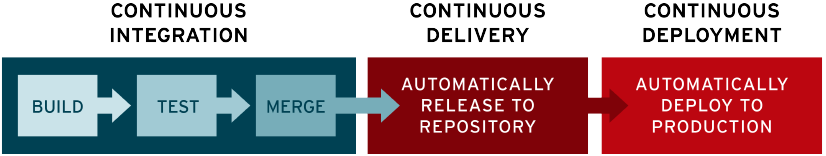
\includegraphics[width=7cm]{image/ci-cd-flow.png}
    \end{frame}

    \begin{frame}
        \frametitle{Histoire du CI/CD}
        \framesubtitle{Une histoire récente d'une vingtaine d'années}
        \transdissolve
        \begin{itemize}
            \item 2005, première version de Hudson, le précurseur de Jenkins par Kohsuke Kawaguchi.
            \item 2010, le terme \textquote{Continuous Integration} est utilisé pour la première fois dans un livre par Jez Humble\footnote{\label{ci}Continuous Delivery, \url{https://www.continuousdelivery.com/}}.
            \item 2011, Jenkins est libéré.
            \item 2024, plus de 38 plateformes mainstream\footnote{38 Best CI/CD Tools For 2024, \url{https://www.lambdatest.com/blog/best-ci-cd-tools/}}.
        \end{itemize}
    \end{frame}

    \begin{frame}
        \frametitle{Les avantages du CI/CD}
        \framesubtitle{Si tout peut être réalisé en local, pourquoi utiliser un serveur~?}
        \transdissolve
        \begin{itemize}
            \item Les plateformes de CI/CD sont avant tout des outils collaboratifs.
            Elles permettent le partage des développements dans l'équipe et dans l'entreprise.
            On peut suivre en direct l'état d'avancement et la qualité des développements de ses collègues.
            \item Elles s'intègre à de nombreux outils comme les SSO, Git, les outils de gestion de projet et de qualité comme ceux d'Atlassian (Jira, Confluence, Bitbucket, etc).
            \item Une UX/UI plus simple que des données un terminal.
            La prise en main peut-être faite par des métiers autre que celui de développeur (Testeur, Release Manager, Hardware).
            \item Permet de partager les ressources hardware requises pour la compilation, les tests, entre des machines plus ou moins disponibles.
            E.g., dans l'embarqué, cela permet de ne pas multiplier le hardware et de limiter le nombre de bancs de test.
            En générale la compilation qui peut prendre beaucoup de ressources CPU et peut être délocalisée sur un serveur dédié.
        \end{itemize}
    \end{frame}

    \begin{frame}
        \frametitle{Les avantages du CI/CD}
        \framesubtitle{Quelles différences avec le DevOps~?}
        \transdissolve
        Le CI/CD est un des outils du DevOps.
        \bigbreak
        C'est l'outil dédié au développement et à la livraison de logiciels de qualité.
        On confond parfois les deux car le terme DevOps étant plus hype que CI/CD, est plus souvent est utilisé.
        \bigbreak
        \centering
        
\includegraphics[width=5cm]{image/caveman-using-a-sophisticated-tool.png}
    \end{frame}

    \begin{frame}
        \frametitle{Le fondamental du CI/CD}
        \framesubtitle{Livre et site web de Jez Humble\cref{ci}}
        \transdissolve
        Jez Humble fait un travaille academic depuis les années 2000 pour mesurer l'impact du CI/CD sur les professionnels de l'IT~.
        \bigbreak
        En plus de plusieurs paramètres liés à la qualité logiciel, il mesure même un impact positif sur l'ambiance de travail~!
        \bigbreak
        Son livre sur le sujet, \textquote{Continuous Delivery}, est une référence dans le domaine.
        Son site web \url{https://www.continuousdelivery.com/} contient déjà beaucoup de ressources.
    \end{frame}

    \begin{frame}
        \frametitle{Le business du CI/CD}
        \framesubtitle{Ce n'est pas une simple technologie mais un marché, attention aux coûts}
        \transdissolve
        Git, Python, que nous avons vu, sont des technologies open source devenues des standard.
        Toutes leurs fonctionnalités sont disponibles gratuitement.
        Contrairement à elles, certaines plateformes de CI/CD sont payantes.
        \bigbreak
        Parmi les business model, on trouve~:
        \begin{itemize}
            \item Le freemium, une version gratuite limitée en fonctionnalités.
            \begin{itemize}
                \item Github est gratuit jusqu'à une certaine consommation de ressources (temps CPU, disque, etc) et est limité en fonctionnalités.
                \item Gradle est toujours \textquote{full featured} en local mais Devlocity, le SAAS qui va avec et rajoute des fonctionnalités est payant.
                \item Gitlab Community Edition VS Entreprise edition.
            \end{itemize}
            \item L'auto-hébergement d'une solution complète open source et le on-premise.
            \begin{itemize}
                \item Jenkins.
            \end{itemize}
            \item Les solutions propriétaires.
            \begin{itemize}
                \item TeamCity est payant en auto-hébergement et on-premise.
                \item Travis CI~.
            \end{itemize}
        \end{itemize}
    \end{frame}

    \begin{frame}
        \frametitle{Les différences entre plateformes}
        \transdissolve
        A lire absolument, un comparatif des différentes plateformes par Atlassian \url{https://www.atlassian.com/fr/continuous-delivery/continuous-integration/tools}.
        \bigbreak
        Les différences sont nombreuses, on peut citer~:
        \begin{itemize}
            \item Certains permettent de créer des clusters sur n'importes quelles machines.
            Par exemple Jenkins avec son cluster formé de \textquote{slave(s)} et d'un \textquote{master}.
            Tout ce qui se passe sur les \textquote{slaves} est visible sur l'IHM du \textquote{master}.
            \item AWS CodePipeline permet d'avoir de multiples nodes mais sur des machines AWS uniquement \emoji{money-mouth-face}.
            \item Devlocity n'a qu'une instance centrale du serveur
            \item Leur communauté, une communauté open source peut développer des plugins, des scripts, des outils, etc, pour virtuellement toutes les applications qui ne sont pas prévues dans la version de base.
            De ce point de vue, Jenkins est dans les premiers.
            \item L'organisation en jobs ou en pipelines de jobs.
        \end{itemize}
    \end{frame}

    \begin{frame}
        \frametitle{Les limites du CI/CD}
        \framesubtitle{Quelles sont les limites du CI/CD~?}
        \transdissolve
        \pause
        \begin{columns}
            \column{0.5\textwidth}
            \begin{itemize}
                \item le coût des licences ou des machines.
                \item Pas de limites sur le type de logiciel, on peut y connecter un banc de test pour l'embarqué et l'IOT, dans le web, la data, etc\ldots
                \item Les ressources des machines disponibles.
                \item La complexité des tests, plus ils sont nombreux et plus ils sont longs à faire tourner et analyser.
            \end{itemize}
            \column{0.5\textwidth}
            \centering
            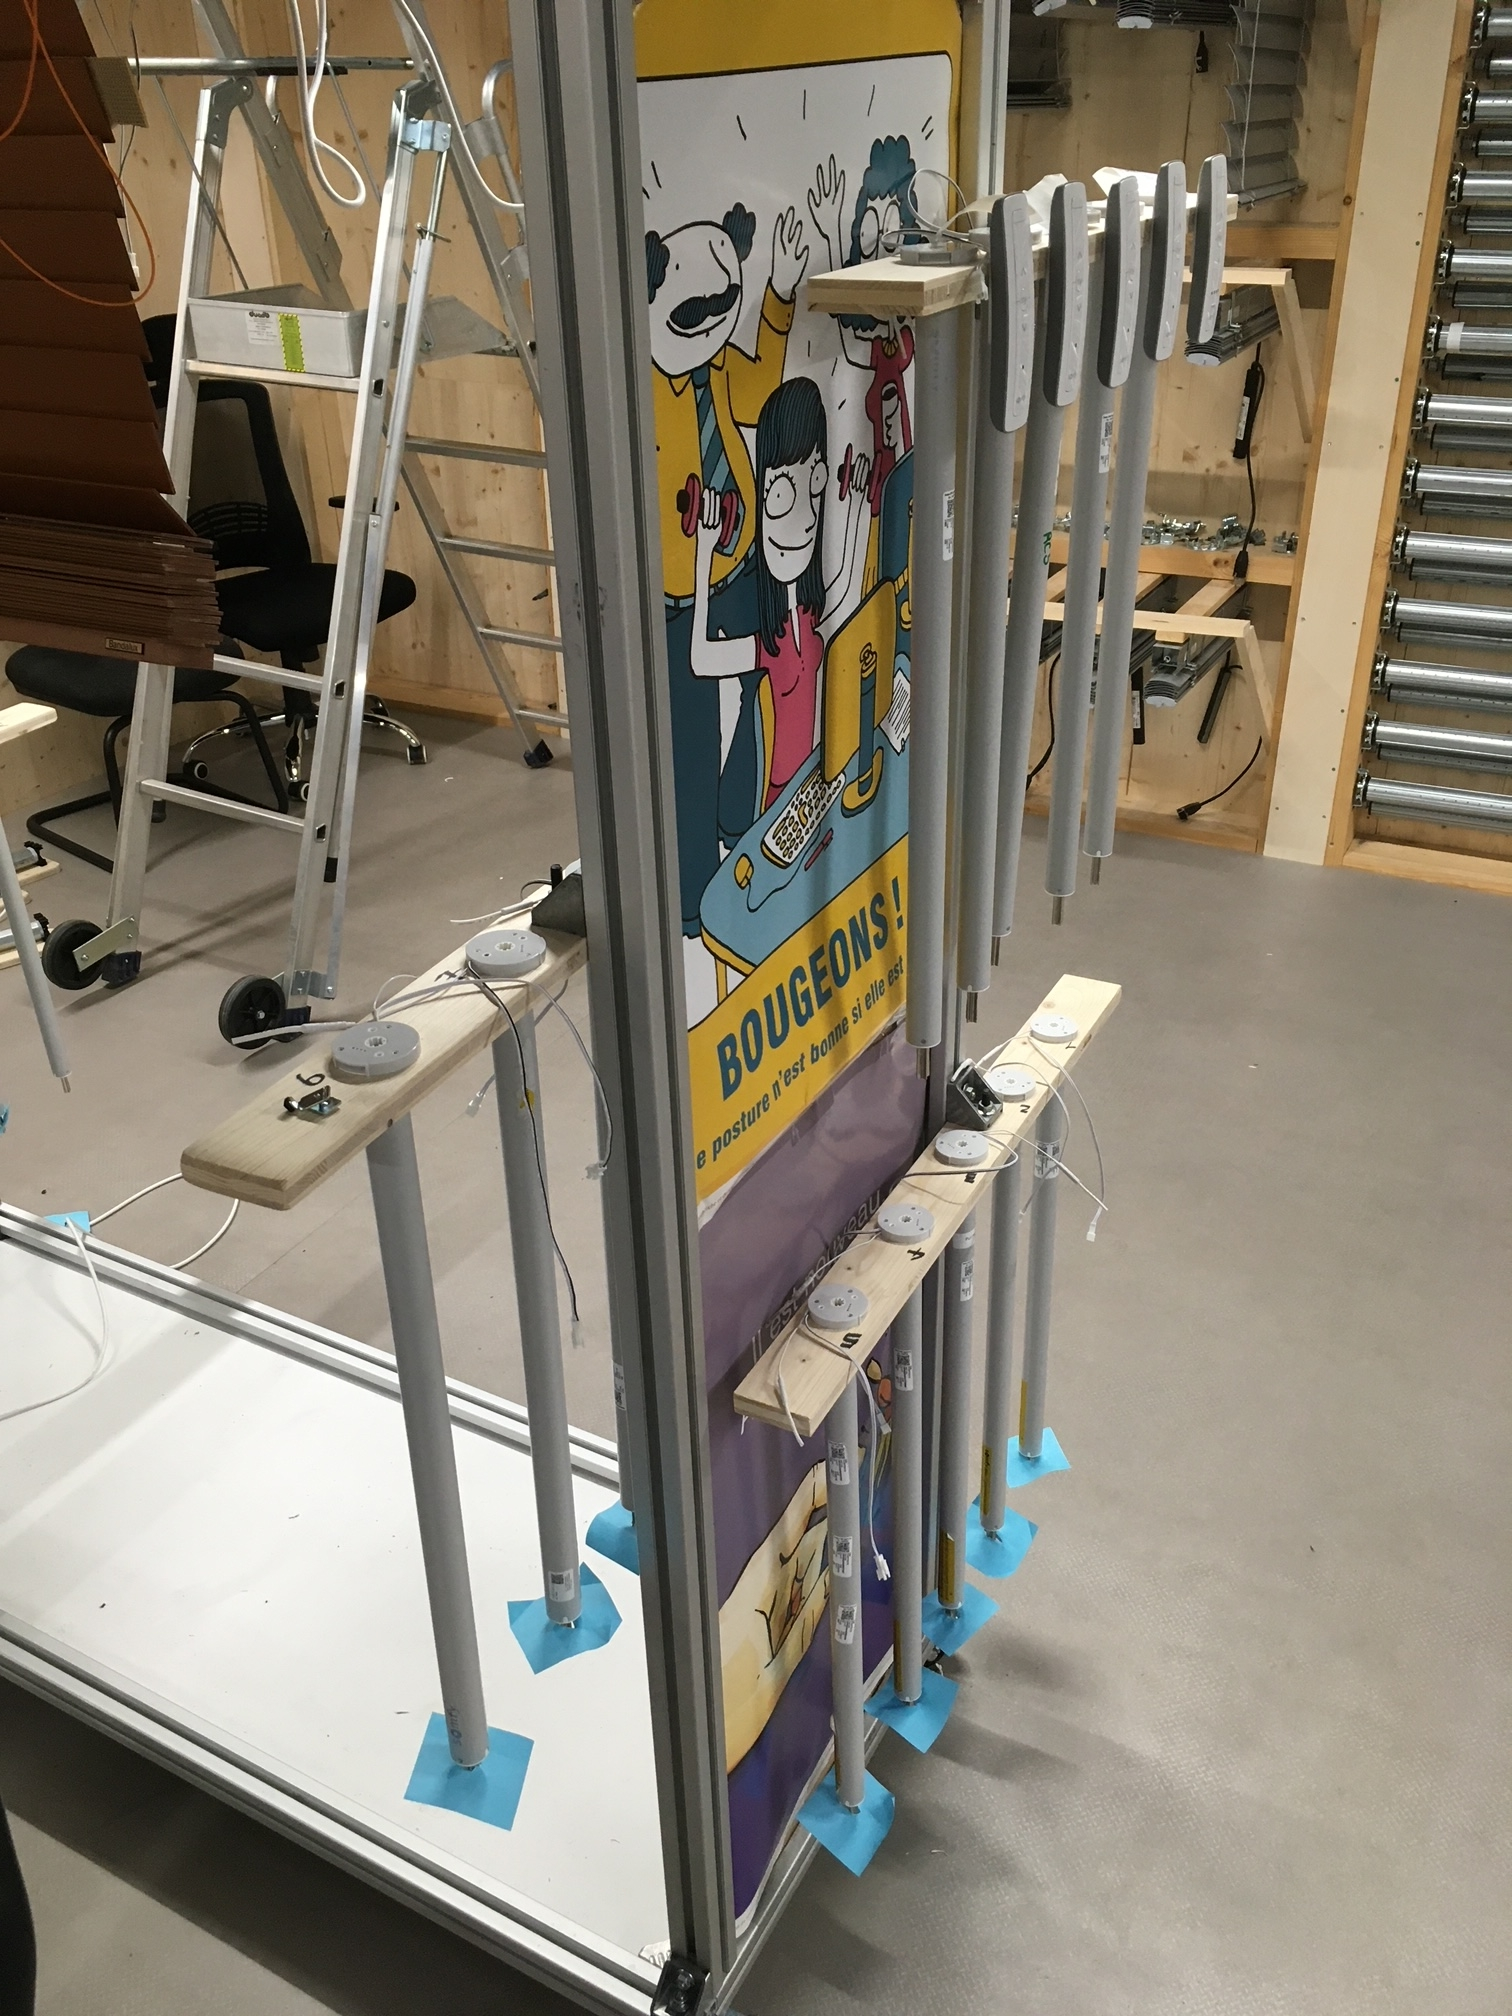
\includegraphics[width=5cm]{image/somfy-test-bench.jpg}
        \end{columns}
    \end{frame}

    \begin{frame}
        \frametitle{Les plateformes les plus utilisées CI/CD}
        \framesubtitle{Résultat de l'enquête JetBrains 2023 sur le CI/CD\footnote{Best Continuous Integration Tools for 2024 ‒ Survey Results, \url{https://blog.jetbrains.com/teamcity/2023/07/best-ci-tools/}}}
        \transdissolve
        \centering
        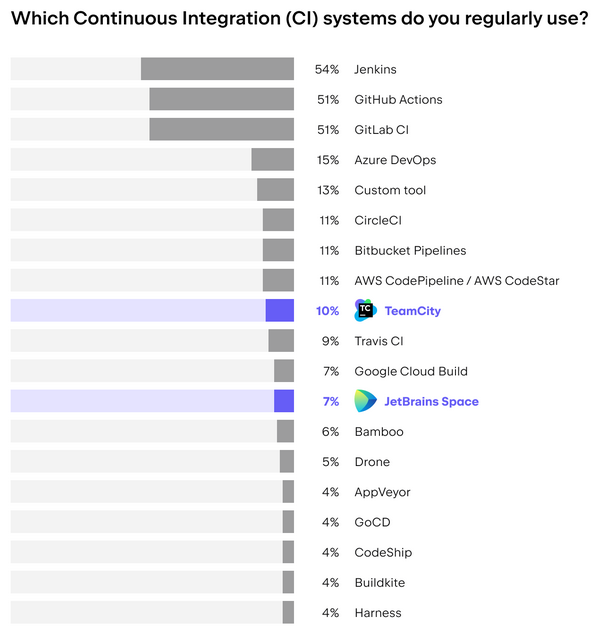
\includegraphics[width=6cm]{image/ci-jetbrains-survey.png}
    \end{frame}

    \begin{frame}
        \frametitle{Exemple de CI/CD}
        \framesubtitle{Exemple de CPython sur GitHub{\footnote{CPython implémentation, \url{https://github.com/python/cpython?tab=readme-ov-file}}} Actions}
        \transdissolve
        Une partie seulement de CPython, l'implémentation classique officielle de Python est sur GitHub, il y en a aussi sur Azure DevOps.
        On y trouve 21 workflows différents~!
        \bigbreak
        \centering
        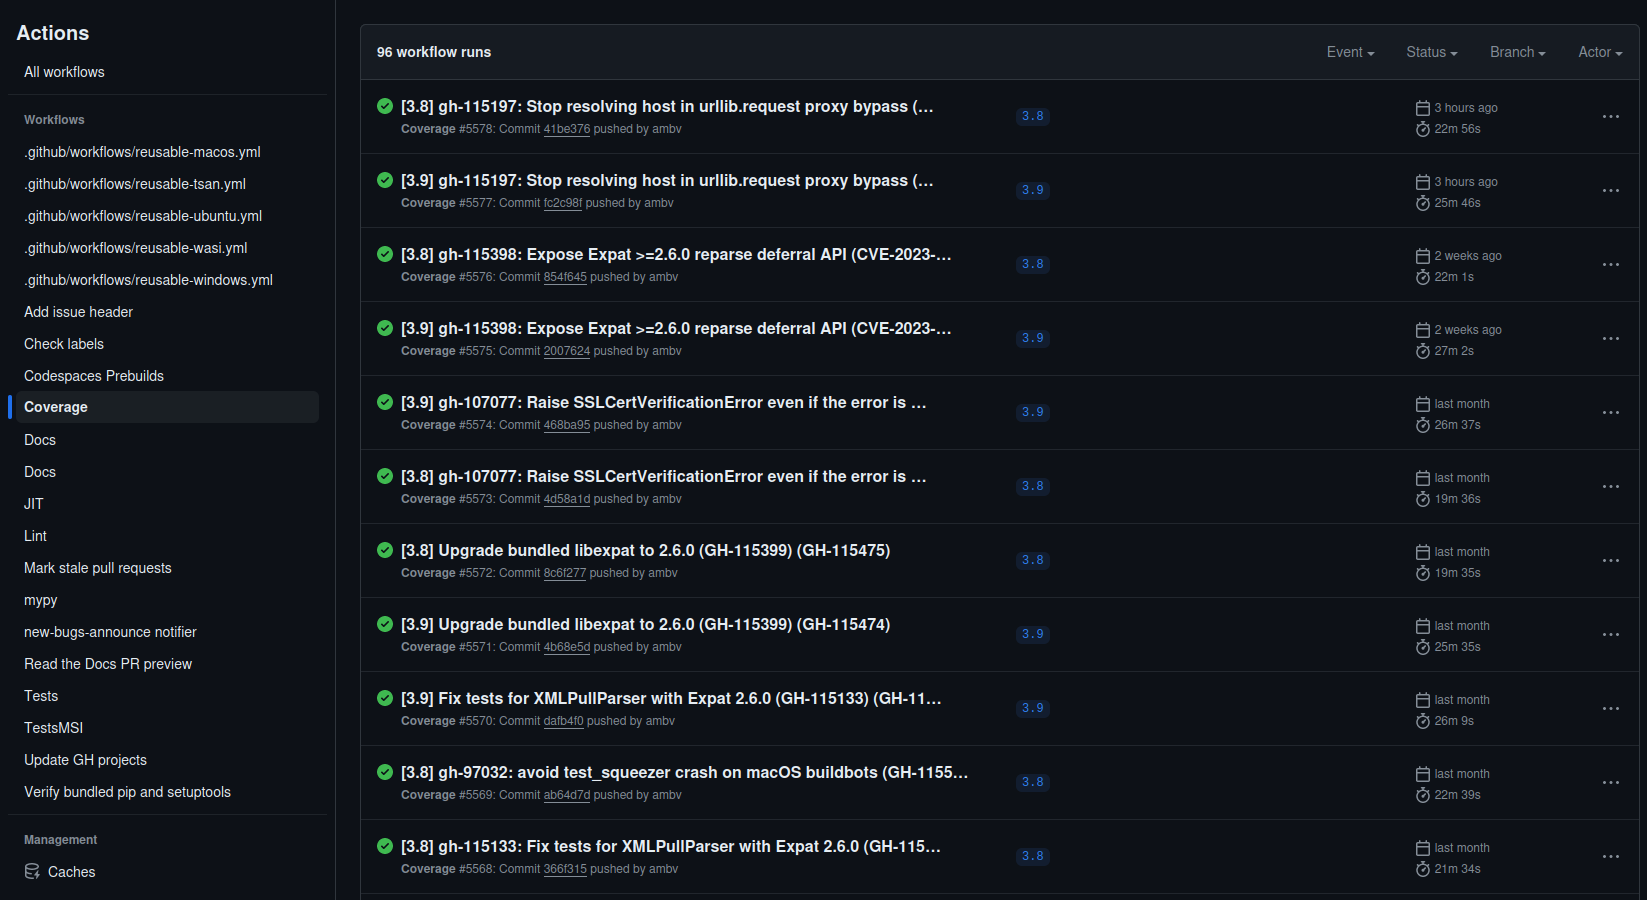
\includegraphics[width=8cm]{image/cpython-github-workflows.png}
    \end{frame}

    \begin{frame}
        \frametitle{Exemple de CI/CD}
        \framesubtitle{Exemple de CPython sur GitHub{\footnote{CPython implémentation, \url{https://github.com/python/cpython?tab=readme-ov-file}}} Actions}
        \transdissolve
        5 workflows \textquote{triggered} par un push et une PR~!
        \bigbreak
        \centering
        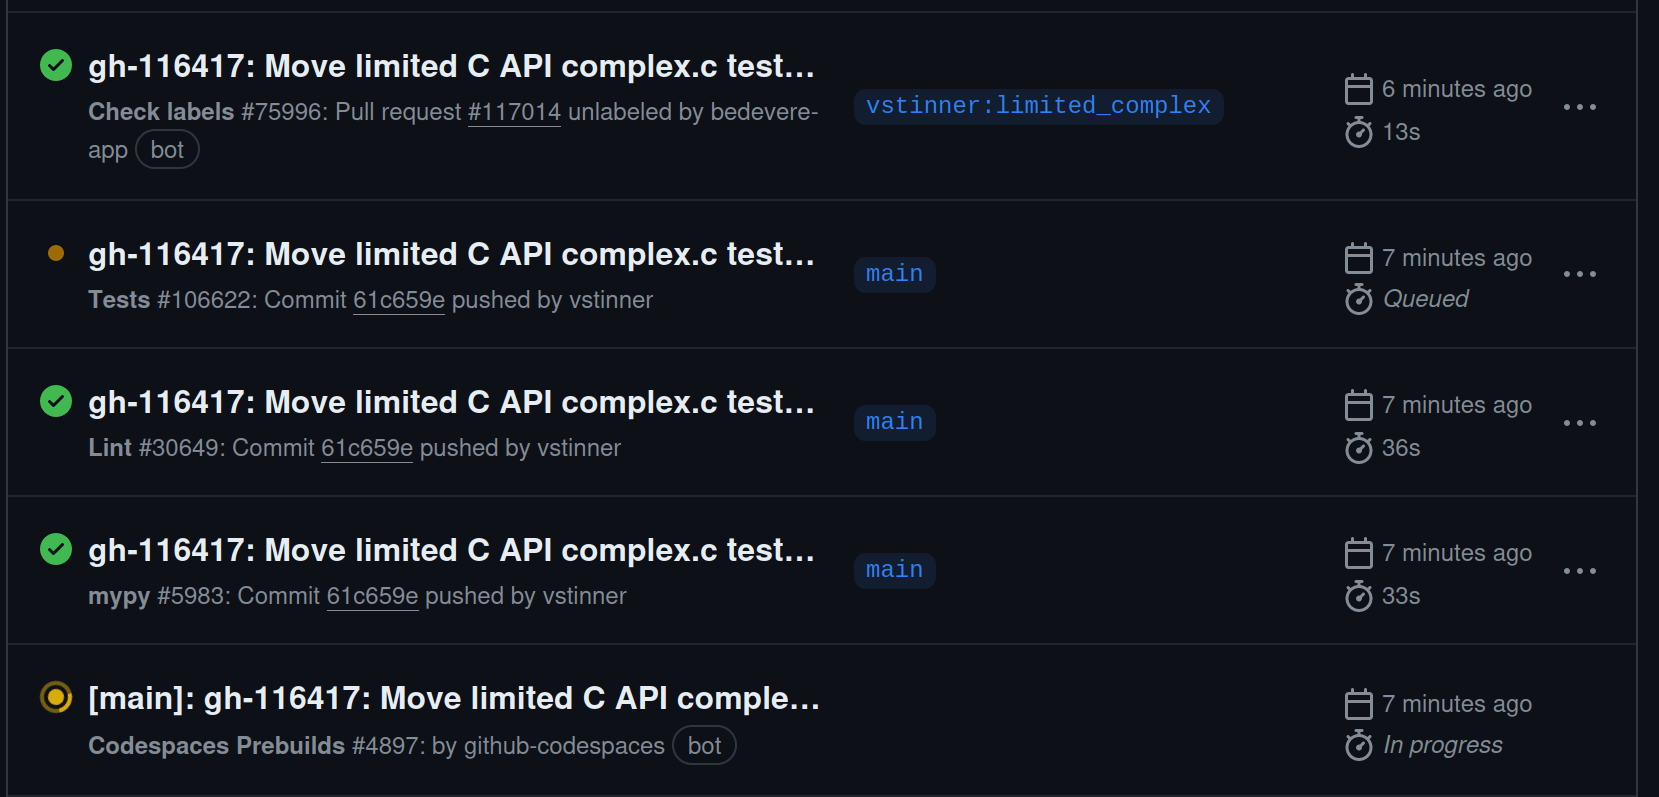
\includegraphics[width=8cm]{image/cpython-actions-triggered.png}
    \end{frame}

    \begin{frame}
        \frametitle{Exemple de CI/CD}
        \framesubtitle{Exemple de CPython sur GitHub{\footnote{CPython implémentation, \url{https://github.com/python/cpython?tab=readme-ov-file}}} Actions}
        \transdissolve
        \begin{columns}
            \column{0.4\textwidth}
            1 seul workflow compte des dizaines de jobs~!
            \bigbreak
            1 seul job compte plusieurs steps~!
            \column{0.6\textwidth}
            \centering
            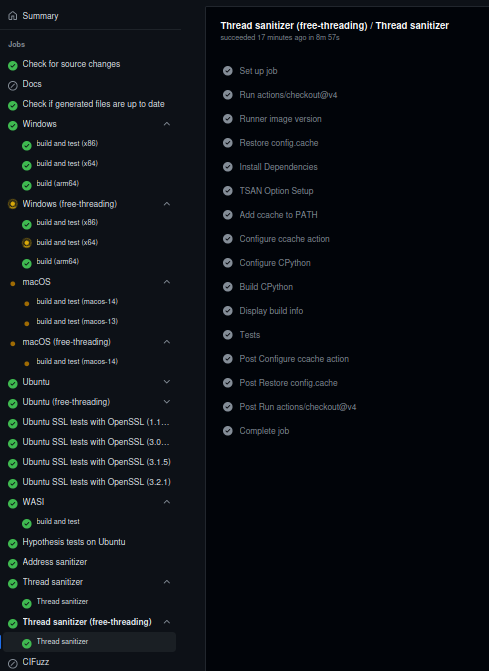
\includegraphics[width=5cm]{image/cpython-workflow-jobs.png}
        \end{columns}
    \end{frame}

    \begin{frame}
        \frametitle{Exemple de CI/CD}
        \framesubtitle{Exemple de worflow GitHub{\footnote{Automate your workflow from idea to production, \url{https://github.com/features/actions}}}}
        \transdissolve

        Definition~:
        \begin{itemize}
            \item Un workflow est une suite de jobs.
            \item Un job est une tache à réaliser.
            \item Un step est une étape de la tache.
            \item Un artefact est un fichier généré par un step.
        \end{itemize}
    \end{frame}

    \begin{frame}
        \frametitle{Exemple de CI/CD}
        \framesubtitle{Exemple de worflow GitHub de ce repository, exercice de 15 minutes}
        \transdissolve
        Que peut-on faire comme workflow, GitHub Actions, etc, sur les dépôts de ce cours~?
        \begin{itemize}
            \item \url{https://github.com/St-Michel-IT/qualite-code-source/}
            \item \url{https://github.com/St-Michel-IT/testing/}
        \end{itemize}
        \bigbreak
        \centering
        
\includegraphics[width=5cm]{image/young-praticing-her-homework.png}
    \end{frame}

    \begin{frame}[fragile]
        \frametitle{Exemple de CI/CD}
        \framesubtitle{Exemple de worflow GitHub de ce repository{\footnote{Worflow de génération des documents à partir de Latex, \url{https://github.com/St-Michel-IT/qualite-code-source/blob/master/.github/workflows/}}}}
        \transdissolve
        Les workflows sont dans les fichiers suivants~:
        \begin{lstlisting}[language=sh]
chrichri@chrichri-HKD-WXX:~/Documents/Campus-St-Michel-IT/qualite-code-source$ tree .github/
.github/
--- workflows
    --- build-document.yml
    --- checkmytex.yml
    --- shell-check.yml
        \end{lstlisting}
        \begin{itemize}
            \item \lstinline{build-document.yml} pour générer le document PDF que vous lisez.
            \item \lstinline{shell-check.yml} pour vérifier la syntaxe des scripts Shell.
            \item \lstinline{checkmytex.yml} pour lister les erreurs dans le fichier LaTex.
        \end{itemize}
    \end{frame}

    \begin{frame}[fragile]
        \frametitle{Exemple de CI/CD}
        \framesubtitle{Exemple de worflow GitHub du repository testing{\footnote{Worflow de génération des documents à partir de Latex, \url{https://github.com/St-Michel-IT/testing/blob/master/.github/workflows/}}}}
        \transdissolve
        Les workflows sont dans les fichiers suivants~:
        \begin{lstlisting}[language=sh]
chrichri@chrichri-HKD-WXX:~/Documents/Campus-St-Michel-IT/testing$ tree .github
.github
--- workflows
    --- build-document.yml
    --- checkmytex.yml
    --- pylint.yml
    --- shell-check.yml
    --- black-formatter.yml
    --- unit-tests.yml
        \end{lstlisting}
        \begin{itemize}
            \item \lstinline{unit-tests.yml} lance les tests avec pytest.
            \item \lstinline{pylint.yml} un linter qui génère un rapport des erreurs et des warnings.
            \item \lstinline{black-formatter.yml} Black formatter qui fait un check sans rien changer.
        \end{itemize}
    \end{frame}

    \begin{frame}
        \frametitle{Exemple de CI/CD}
        \framesubtitle{Pas de runner officiel des worfkflows GitHub en local}
        \transdissolve
        Tout les workflows doivent tourner sur des machines GitHub.
        Avec les coûts et la latence que cela implique.
        \bigbreak
        Quelles sont donc les bonnes pratiques pour éviter les pièges des plateformes comme GitHub, Circle CI, Jenkins, etc~?
        \pause
        \begin{itemize}
            \item Éviter des fonctionnalités propres à ces plateformes.
            C'est à dire agnostiques aux plateforme.
            \item Écrire des scripts qui peuvent être exécutés en local.
            Par exemple (scripts BASH, scripts PowerShell, scripts Gradle\footnote{\label{gradle}Accelerate developer productivity, \url{https://gradle.org/}}, Dockerfiles, scripts Ansible)
            \item Ces scripts peuvent-être appelés dans les jobs du CI/CD~.
            \item Nettoyer vos environnements après le build pour économiser les ressources.
        \end{itemize}
    \end{frame}

    \begin{frame}
        \frametitle{Gradle}
        \framesubtitle{Gradle comme une passerelle entre le local et la plateforme de CI/CD}
        \transdissolve
        Gradle\cref{gradle} est un outil de build open source.
        On script en Groovy\footnote{\label{groovy}Groovy, A multi-faceted language for the Java platform, \url{https://groovy-lang.org/}} ou Kotlin\footnote{Kotlin, \url{https://kotlinlang.org/}}, en local des taches de build, équivalente au jobs des plateformes de CI/CD~.
        \bigbreak
        On débug en local, on teste en local, on commit en local.
        Cela fait gagner un temps considérable (pas de commit/push\ldots) dans le développement du CI/CD~.
        Et donc, cela fait également économiser des ressources de CI/CD~.
        \begin{dangercolorbox}
            Toutes les plateformes de CI/CD ont un plugin/workflow Gradle.
            La portabilité est donc assurée.
        \end{dangercolorbox}
    \end{frame}

    \begin{frame}
        \frametitle{Les marketplaces des plateformes de CI/CD}
        \framesubtitle{Un \textquote{market} gratuit ou payant}
        \transdissolve
        Ne pas avoir peur du nom marketplace, beaucoup de plugins Jenkins ou de workflows GitHub sont gratuits.
        \begin{columns}
            \column{0.5\textwidth}
            \begin{itemize}
                \item Plus de 1~900 plugin Jenkins\footnote[frame]{Jenkins Plugins, \url{https://plugins.jenkins.io/}}.
                \item Plus de 22~000 actions GitHub\footnote[frame]{GitHub Actions, \url{https://github.com/marketplace?type=actions}}.
            \end{itemize}
            \column{0.5\textwidth}
            \centering
            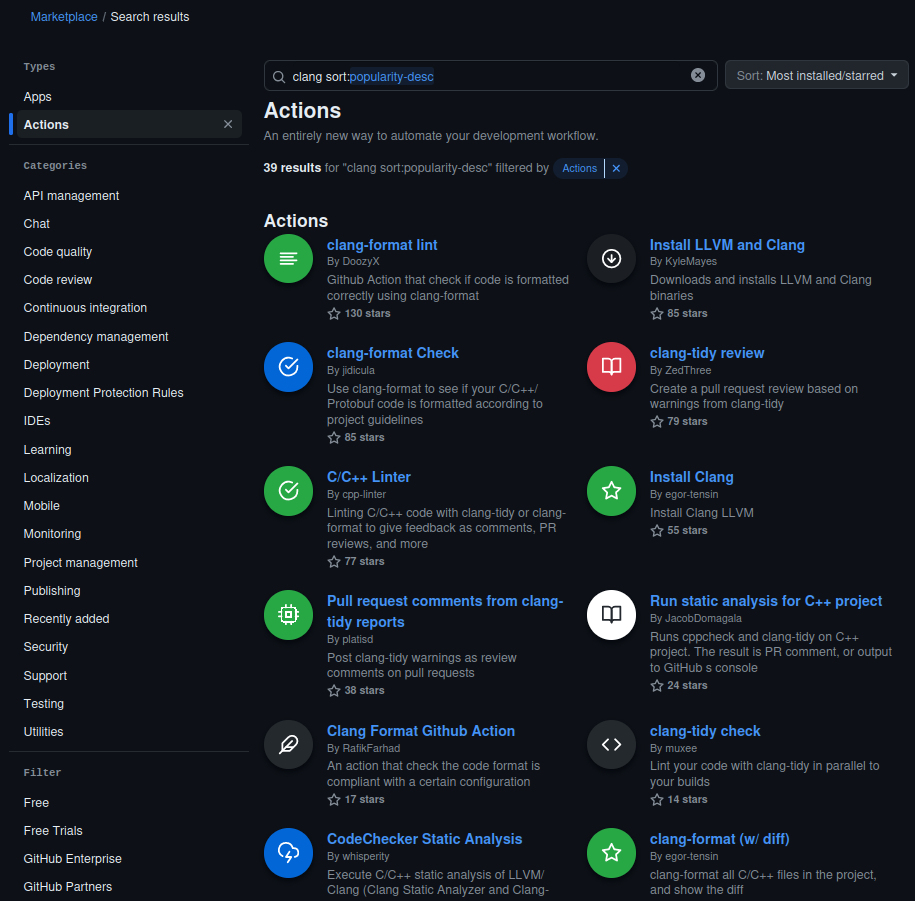
\includegraphics[width=5cm]{image/github-marketplace.png}
        \end{columns}
        Ils sont essentiels pour développer plus rapidement les jobs (reuse, comme dans n'importe quel code).
    \end{frame}

    \subsection{GitHub Action}\label{subsec:github-action}
    \begin{frame}
        \frametitle{Les exemples de CI/CD dans le développement d'API}
        \framesubtitle{Grâce à Swagger et OpenAPI}
        \transdissolve
        Swagger est un fichier de définition d'une API~.
        Il est écrit en YAML ou en JSON. Et les données pour décrire l'API sont dans la OpenAPI Specification\footnote{API Development for Everyone\url{https://swagger.io/}}.
        \break
        \centering
        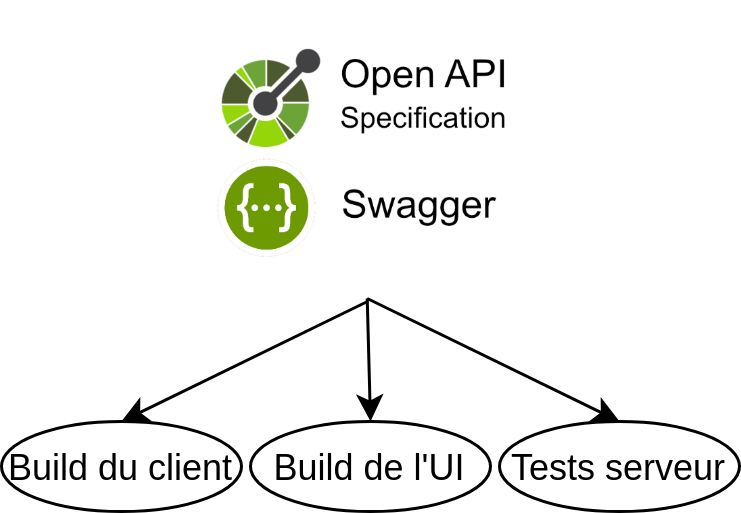
\includegraphics[width=6cm]{image/swagger-capacity.drawio.png}
    \end{frame}

    \begin{frame}[fragile]
        \frametitle{Les exemples de CI/CD dans le développement d'API}
        \framesubtitle{Grâce à Swagger et OpenAPI}
        \transdissolve
        \begin{lstlisting}
/lists:
    get:
      summary: Gets all available data lists.
      description: Returns all custom data lists available to the current user.
      tags:
        - Lists
      responses:
        200:
          description: 'OK'
          content:
            application/json:
              schema:
                type: array
                items:
                  # Reuse du schema de DataList !
                  $ref: '#/components/schemas/DataList'
        401:
          # Reuse des responses !
          $ref: '#/components/responses/Unauthorized'
        5XX:
          $ref: '#/components/responses/ServerError'
        \end{lstlisting}
    \end{frame}

    \begin{frame}
        \frametitle{Les exemples de CI/CD dans le développement d'API}
        \framesubtitle{Une UI pour découvrir l'API}
        \transdissolve
        L'UI est un espace convivial pour découvrir l'API~.
        Il fait aussi office de documentation.
        Par exemple \url{https://api.recherche-entreprises.fabrique.social.gouv.fr/\#/Recherche/search}.
        \bigbreak
        \centering
        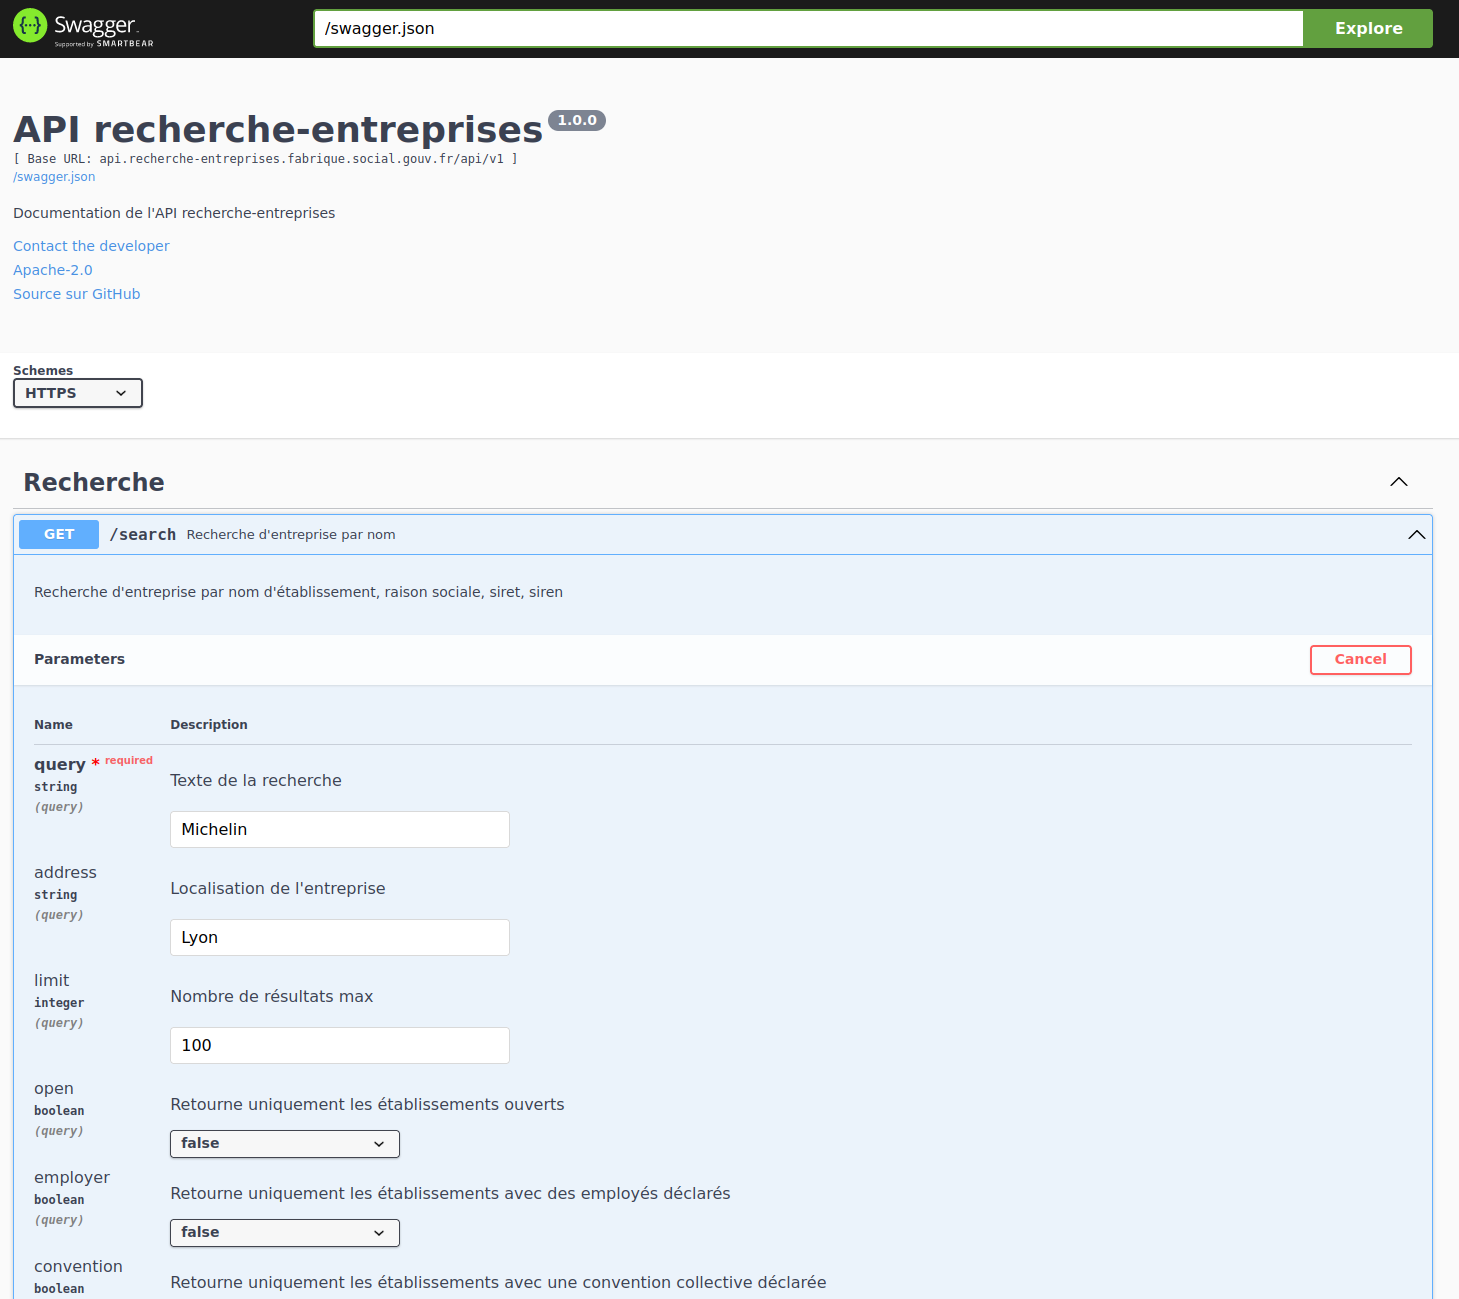
\includegraphics[width=8cm]{image/swagger-ui.png}
    \end{frame}

    \begin{frame}
        \frametitle{Les exemples de CI/CD dans le développement d'API}
        \framesubtitle{Toutes les fonctionnalités sont déjà dans la marketplace (ou les plugins pour Jenkins)}
        \transdissolve
        \centering
        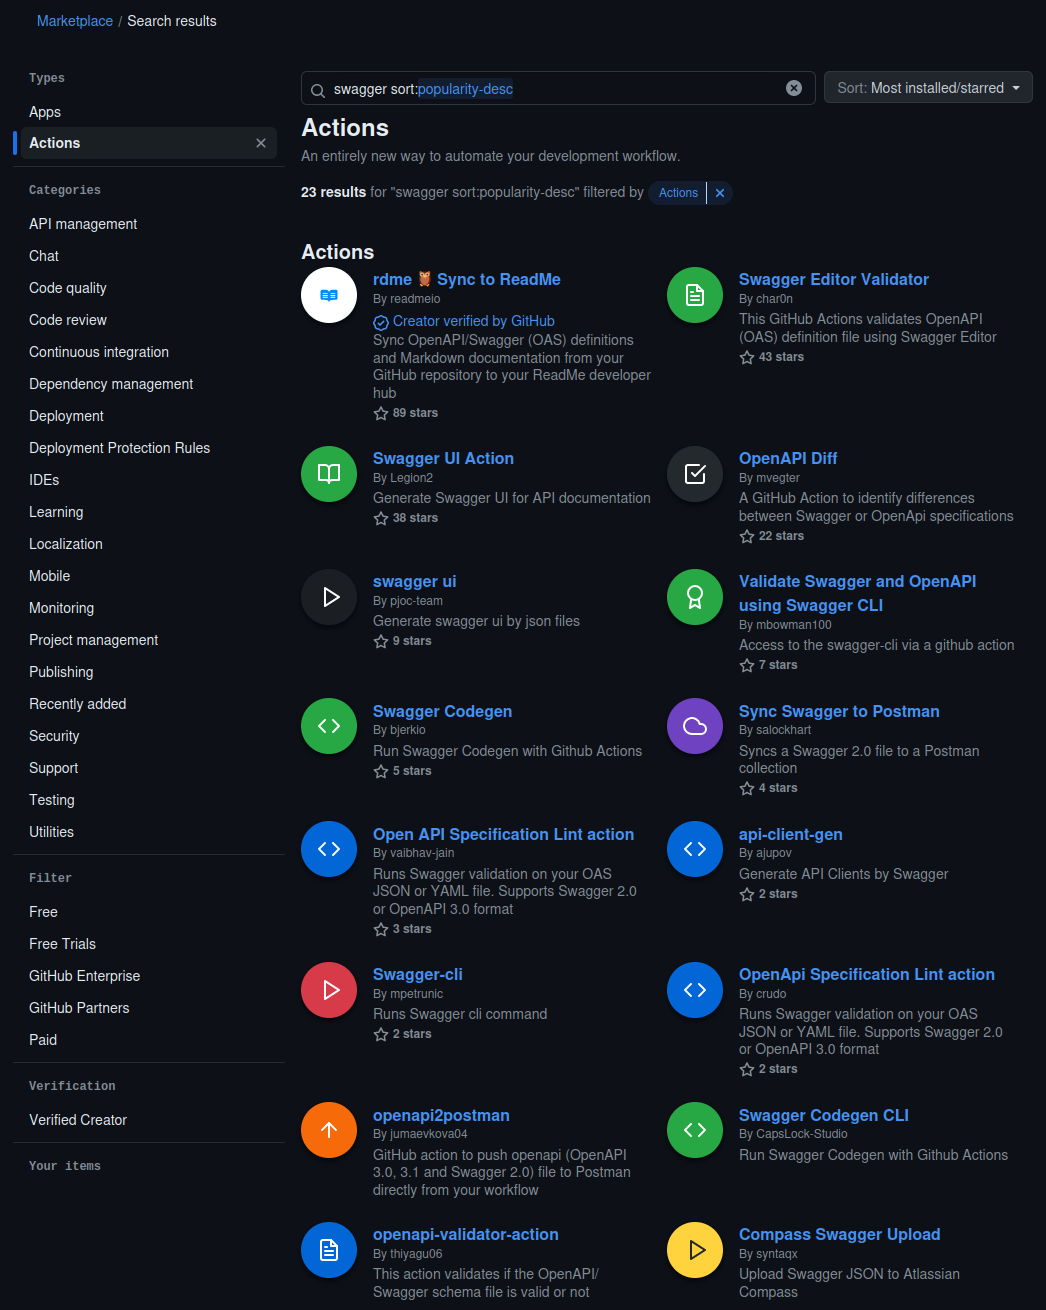
\includegraphics[width=8cm]{image/swagger-worflows.png}
    \end{frame}

    \begin{frame}[fragile]
        \frametitle{Les exemples de CI/CD avec le déploiement d'une image Docker}
        \framesubtitle{GitHub ou Docker Hub peuvent héberger des images Docker\footnote{Publishing Docker images, \url{https://docs.github.com/en/actions/publishing-packages/publishing-docker-images}}}
        \transdissolve
        \begin{lstlisting}
      - name: Log in to Docker Hub
        uses: docker/login-action@f4ef78c080cd8ba55a85445d5b36e214a81df20a
        with:
          username: ${{ secrets.DOCKER_USERNAME }}
          password: ${{ secrets.DOCKER_PASSWORD }}
      - name: Extract metadata (tags, labels) for Docker
        id: meta
        uses: docker/metadata-action@9ec57ed1fcdbf14dcef7dfbe97b2010124a938b7
        with:
          images: my-docker-hub-namespace/my-docker-hub-repository
      - name: Build and push Docker image
        uses: docker/build-push-action@3b5e8027fcad23fda98b2e3ac259d8d67585f671
        with:
          context: .
          file: ./Dockerfile
          push: true
          tags: ${{ steps.meta.outputs.tags }}
          labels: ${{ steps.meta.outputs.labels }}
        \end{lstlisting}
    \end{frame}

    \begin{frame}[fragile]
        \frametitle{Les exemples de CI/CD avec la publication de builds}
        \framesubtitle{Pour publier un soft compilé ou packagé sur sa page du dépôt GitHub\footnote{Create Release, \url{https://github.com/marketplace/actions/create-release}}}
        \transdissolve
        \begin{lstlisting}
name: Releases

on:
  push:
    tags:
    - '*'

jobs:

  build:
    runs-on: ubuntu-latest
    permissions:
      contents: write
    steps:
    - uses: actions/checkout@v3
    - uses: ncipollo/release-action@v1
      with:
        artifacts: "release.tar.gz,foo/*.txt"
        bodyFile: "body.md"
        \end{lstlisting}
    \end{frame}

    \begin{frame}
        \frametitle{Les exemples de CI/CD avec la publication de builds}
        \framesubtitle{Publication de VS Code packagé\footnote{microsoft/vscode, \url{https://github.com/microsoft/vscode/releases}}}
        \transdissolve
        \centering
        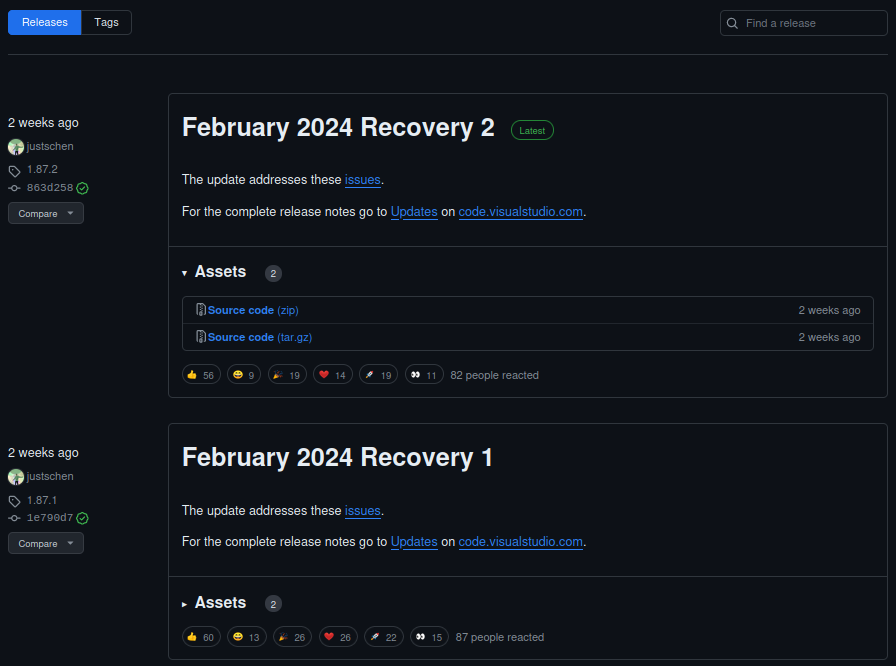
\includegraphics[width=9cm]{image/vs-code-release.png}
    \end{frame}

    \begin{frame}
        \frametitle{Quelques exemples d'étapes de compilation du CI/CD}
        \framesubtitle{Quelles types de jobs pour passer d'un code source à un exécutable?}
        \transdissolve
        \pause
        \begin{itemize}
            \item Compilation de C/C++ en binaire avec GCC et Vagrant pour cibler plusieurs les architectures.
            \item Compilation de Python en bytecode.
            \item Compilation de Java en Jar.
            \item Packaging de NodeJS en NPM~.
            \item Packaging de Python en Wheel.
            \item Compiler LaTex en PDF~.
            \item etc\ldots
        \end{itemize}
    \end{frame}

    \subsection{Jenkins}\label{subsec:jenkins}
    \begin{frame}
        \frametitle{Quelques notions de base de Jenkins}
        \framesubtitle{Les jobs VS les pipelines}
        \transdissolve
        Les jobs sont des taches unitaires.

        Un job est plus simple, c'est principalement un ensemble de commandes de \textquote{build}.

        Ce sont des commandes shell, console ou PowerShell en fonction de l'environnement.

        \bigbreak
        Les pipelines sont des enchainements de jobs.
        Le pipeline est écrit en Groovy\cref{groovy} et mais le principe est similaire au fichier Gradle ou workflow GitHub\footnote{Pipeline Examples, \url{https://www.jenkins.io/doc/pipeline/examples/}}.
        \bigbreak
        \centering
        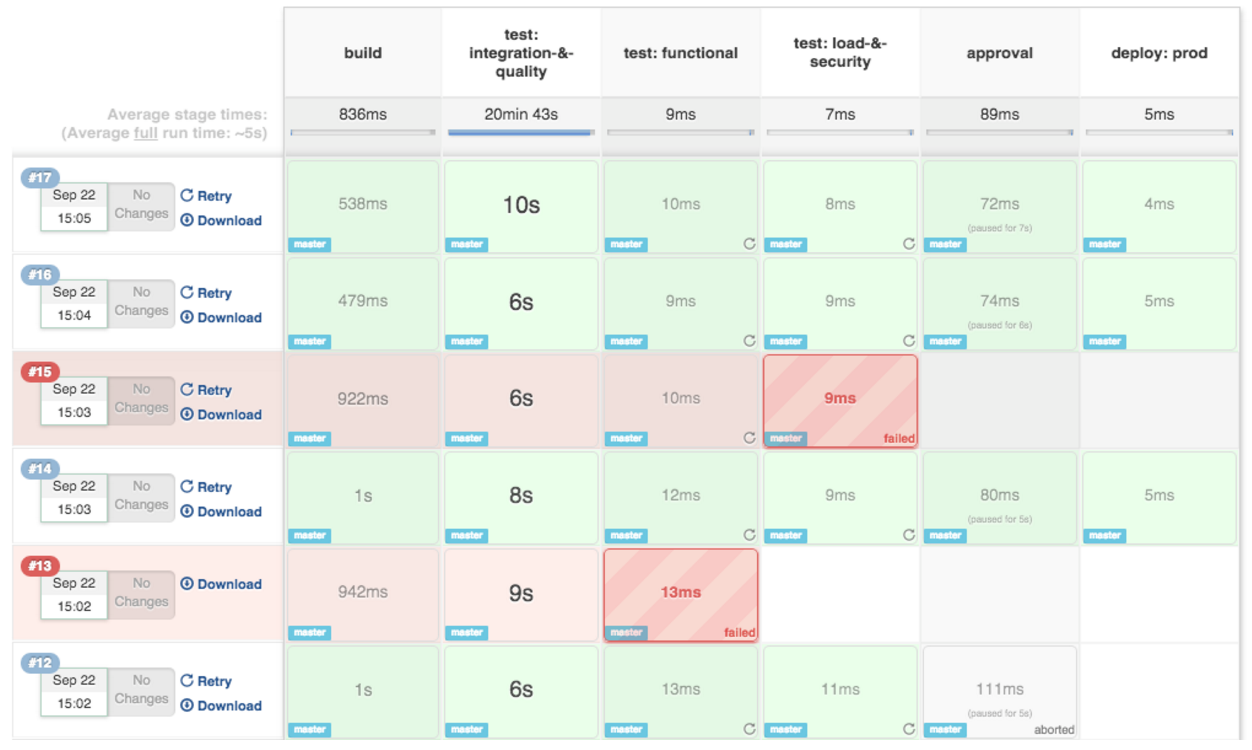
\includegraphics[width=5cm]{image/jenkins-pipeline.png}
    \end{frame}

    \begin{frame}
        \frametitle{Quelques notions de base de Jenkins}
        \framesubtitle{Exemple de pipeline avec Gradle}
        \transdissolve
        Pour être agnostique à une plateforme de CI/CD, on peut exécuter dans la plateforme de CI/CD un build Gradle.

        Jenkins, comme les autres plateformes, permet évidement de faire cela dans les builds ou les pipelines\footnote{Jenkins Gradle plugin, \url{https://plugins.jenkins.io/gradle/}}.
        \bigbreak
        Si un maximum de taches, d'intelligence, de scripting sont dans le build Gradle, il sera plus simple de changer de plateforme de CI/CD~.
    \end{frame}

    \begin{frame}
        \frametitle{Quelques notions de base de Jenkins}
        \framesubtitle{Les clusters de slaves et master\footnote{Jenkins master-slave setup, \url{https://www.linkedin.com/pulse/jenkins-slave-node-soma-sekhar-k-gusdc/}}}
        \transdissolve
        Différentes machines esclaves peuvent être reliées à une machine maître.
        Soit pour répartir la charge, soit pour avoir des machines avec des environnements ou des configurations différentes.
        Ce sont des Jenkins slave agents aussi appelés node.
        \bigbreak
        \centering
        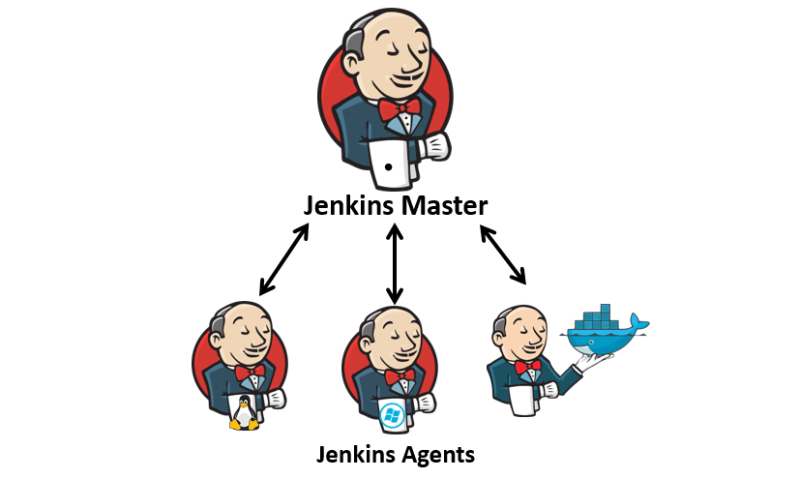
\includegraphics[width=5cm]{image/jenkins-cluster.png}
    \end{frame}

    \subsection{GitLab CI}\label{subsec:gitlab-ci}

    \begin{frame}
        \frametitle{GitLab}
        \framesubtitle{Histoire et présentation de GitLab\footnote{What we do, \url{https://about.gitlab.com/company/}}\footnotestep\footnote{GitLab, \url{https://gitlab.com/st-michel/}}}
        \transdissolve
        GitLab est une plateforme de gestion de développement de logiciels au sens large.
        Son développement à commencé en 2011~.
        \bigbreak
        Le nombre de ces fonctionnalité ne cesse d'augmenter mais elle est surtout connue comme VCS pour son intégration de Git.
        \bigbreak
        GitLab se tourne vers le CI/CD en 2018.
        \bigbreak
        Mais on y trouve encore de nombreuses autres fonctionnalités~:
        \begin{itemize}
            \item Gestion de projet
            \item Bug tracking
            \item WiKi
            \item Many more\ldots
        \end{itemize}
    \end{frame}

    \begin{frame}
        \frametitle{GitLab}
        \framesubtitle{Les versions}
        \transdissolve
        Community ou Entreprise Edition~:
        \bigbreak
        \centering
        
\includegraphics[width=8cm]{image/gitlab-versions}
        \flushleft
        La version CE est à installer sur une de ses propres machines.

        La version EE se décline en Premium et Ultimate.

        Les fonctionnalités de ces 3 versions sont bien différentes, voir \url{https://about.gitlab.com/pricing/feature-comparison/}.

        On ne paye donc pas que pour les ressources utilisés comme chez GitHub mais aussi pour les fonctionnalités.
    \end{frame}

    \begin{frame}
        \frametitle{GitLab}
        \framesubtitle{Les versions}
        \transdissolve
        Community ou Entreprise Edition~:
        \bigbreak
        \centering
        
\includegraphics[width=8cm]{image/gitlab-versions}
        \flushleft
        La version CE est à installer sur une de ses propres machines.

        La version EE se décline en Premium et Ultimate.

        Les fonctionnalités de ces 3 versions sont bien différentes, voir \url{https://about.gitlab.com/pricing/feature-comparison/}.

        On ne paye pas donc que pour les ressources utilisés comme chez GitHub mais aussi pour les fonctionnalités.
    \end{frame}

    \begin{frame}[fragile]
        \frametitle{GitLab}
        \framesubtitle{Le pipeline\footnote{Tutorial: Create and run your first GitLab CI/CD pipeline, \url{https://docs.gitlab.com/ee/ci/quick_start/}}}
        \transdissolve
        Très similaire aux workflows GitHub c'est un ensemble de \textquote{Jobs} spécifiés dans un fichier YAML~.
        \bigbreak
        Il doit être à la racine du projet et se nommer \lstinline{.gitlab-ci.yml}.
        \begin{lstlisting}[basicstyle=\ttfamily\tiny]
stages:
  - build
  - test

job_build:
  stage: build
  script:
    - echo "Building the project"

job_test:
  stage: test
  script:
    - echo "Running tests"
        \end{lstlisting}
        Ce Pipeline doit être exécuté dans un runner.
    \end{frame}

    \begin{frame}
        \frametitle{GitLab}
        \framesubtitle{Développement du pipeline dans la web UI de GiLab.com}
        \transdissolve
        La web UI de GitLab permet de développer le pipeline et de valider la syntaxe en live dans le \textquote{Pipeline editor}~:
        \bigbreak
        \centering
        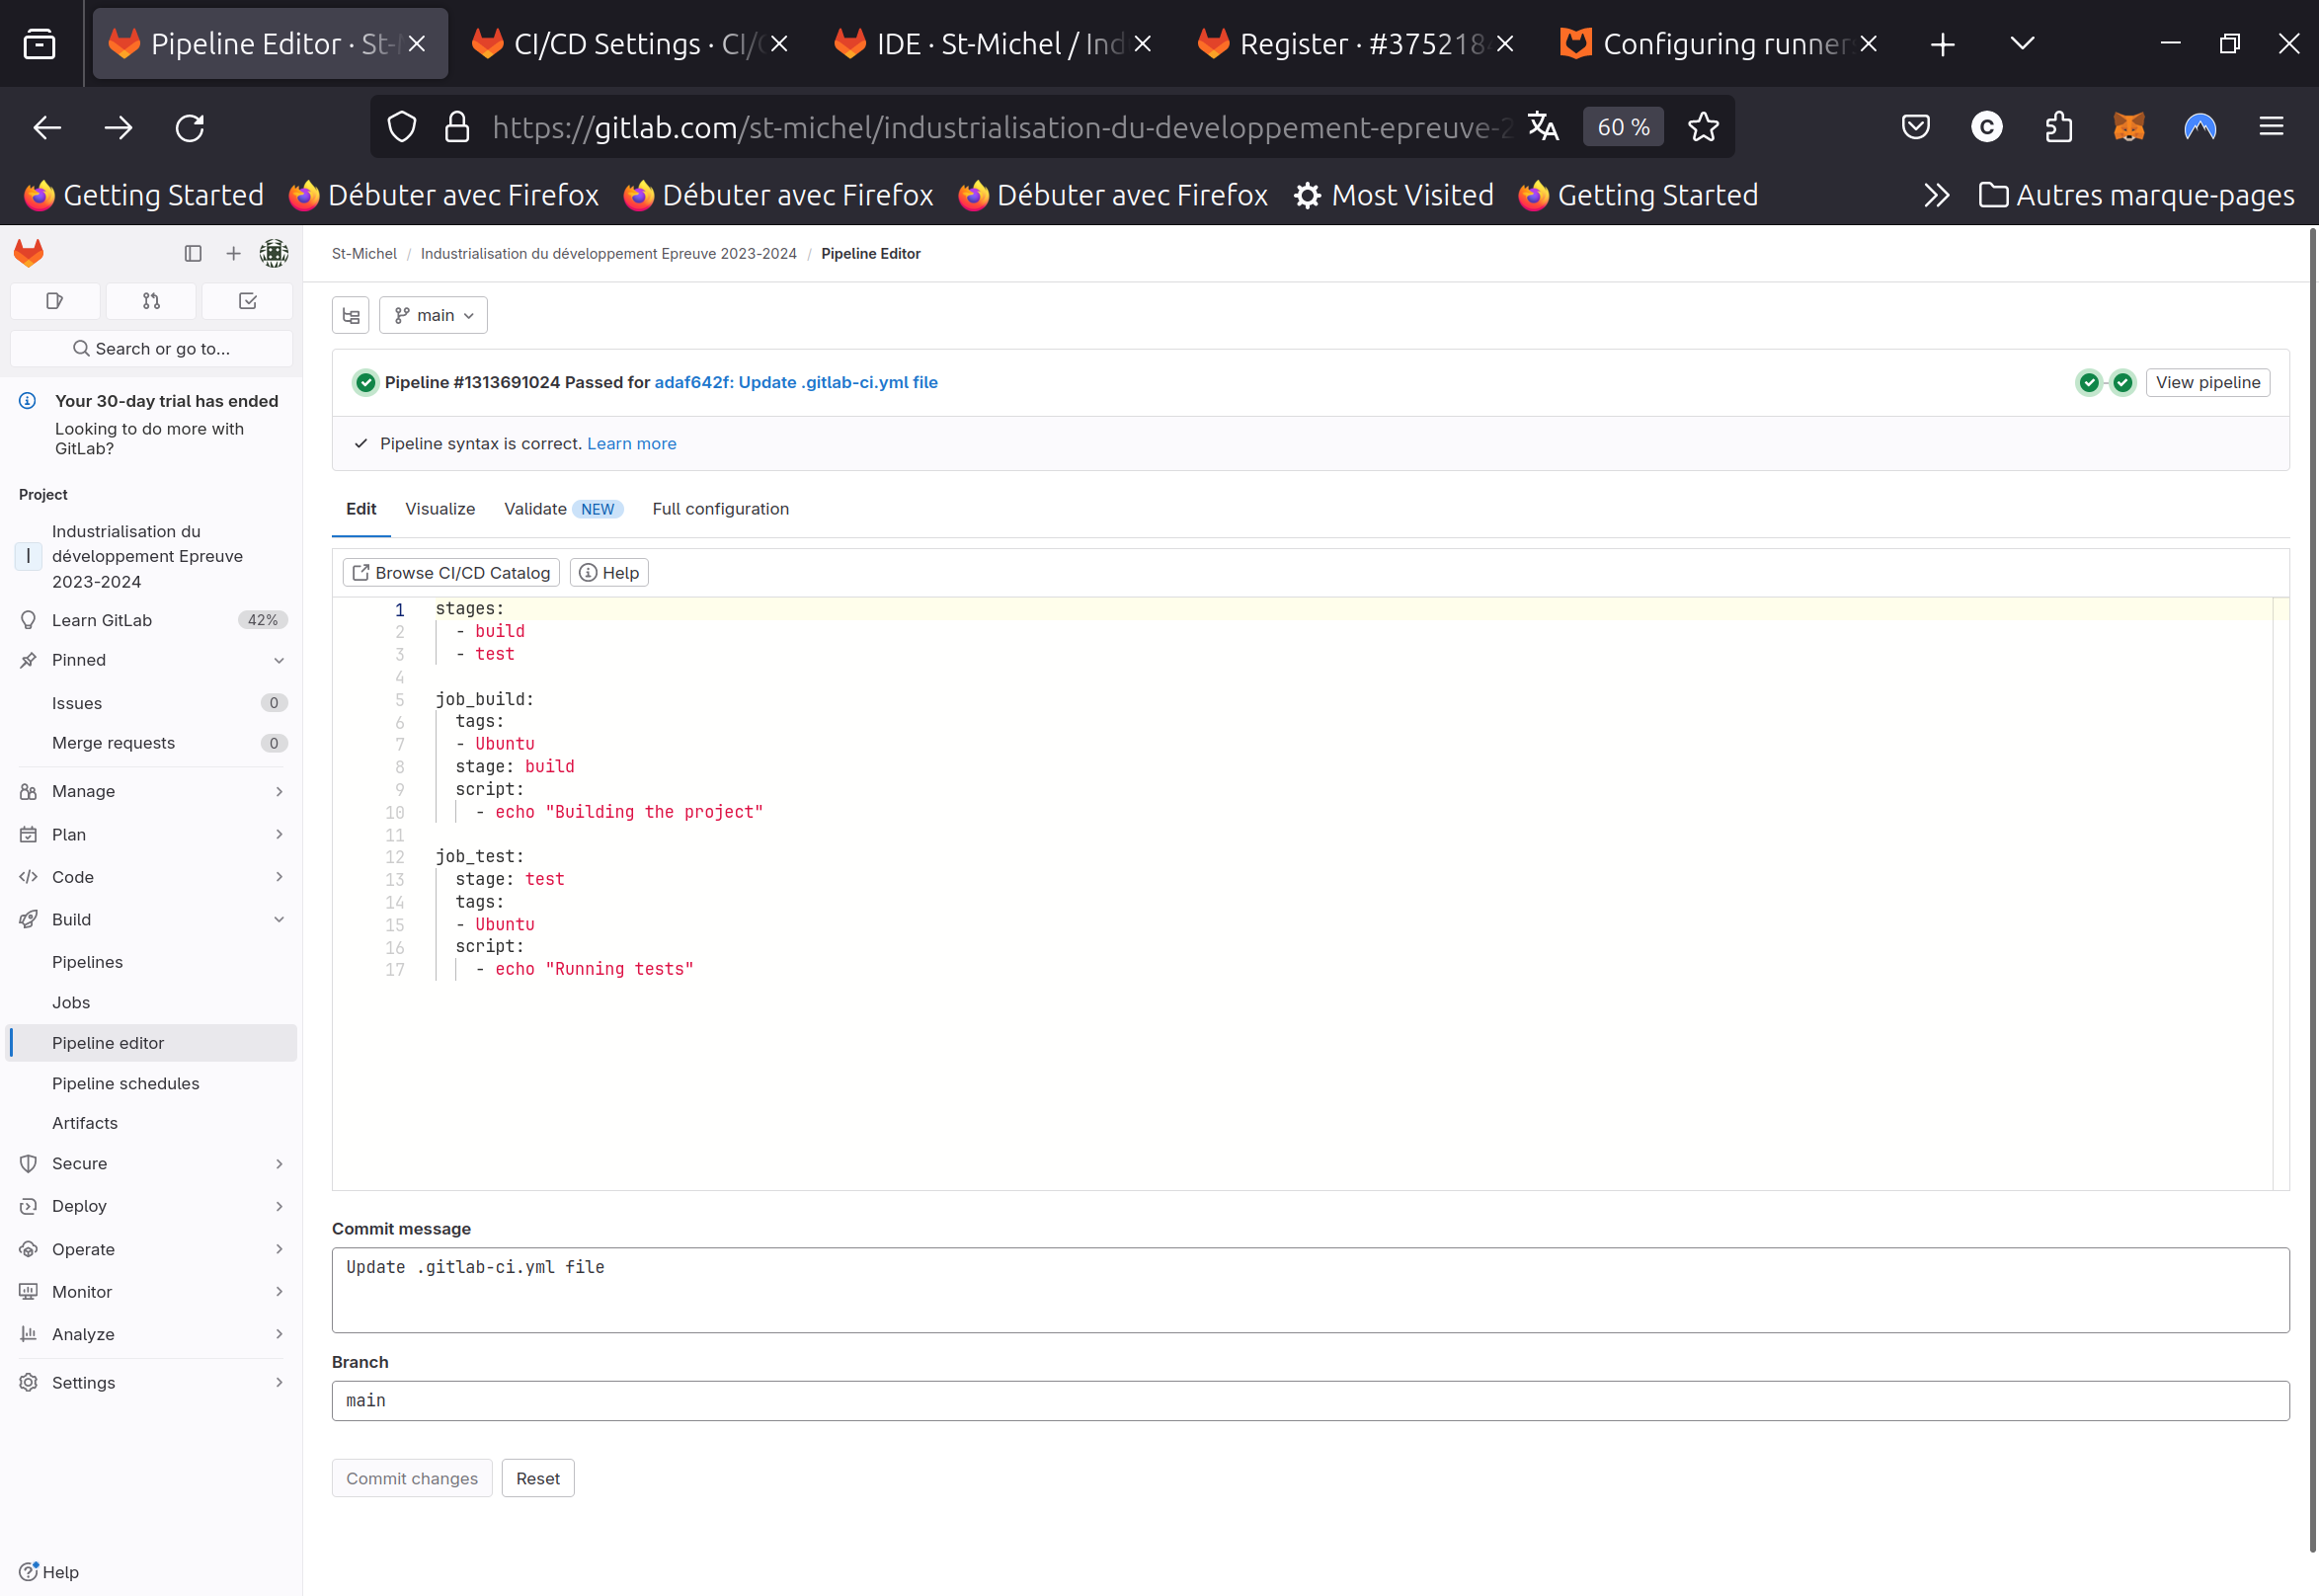
\includegraphics[width=8cm]{image/gitlab-pipeline-editor.png}
    \end{frame}

    \begin{frame}
        \frametitle{GitLab}
        \framesubtitle{Le runner\footnote{\label{configrunner}Tutorial: Create, register, and run your own project runner, \url{https://docs.gitlab.com/ee/tutorials/create\_register\_first\_runner/index.html}}}
        \transdissolve
        Le \textquote{runner} est l'équivalent du Jenkins Slave.
        \bigbreak
        \begin{columns}
            \column{0.5\textwidth}
            Il peut fonctionner via de nombreuses interfaces~:
            \begin{tiny}
                \begin{itemize}
                    \item SSH
                    \item Shell
                    \item VirtualBox
                    \item Docker
                    \item Kubernetes
                    \item \ldots
                \end{itemize}
            \end{tiny}
            \column{0.5\textwidth}
            La machine peut-être un PC, un serveur, un banc de test, Windows, Mac, Linux, etc.
            \bigbreak
            Suivre le tutoriel officiel\cref{configrunner} pour configurer un runner et le lancer.
            Une fois que le programme \lstinline{gitlab-runner run} est lancé, le runner est prêt à exécuter les pipelines.
        \end{columns}
        \begin{dangercolorbox}
            À paramétrer comme service pour qu'il tourne en permanence en tâche de fond.
        \end{dangercolorbox}
    \end{frame}

    \begin{frame}[fragile]
        \frametitle{GitLab}
        \framesubtitle{Exécution d'un pipeline sur un runner donné}
        \transdissolve
        Par défaut si dans le pipeline, aucun runner n'est spécifié, le pipeline est exécuté sur un runner disponible et compatible sans que l'on puisse prédire lequel.
        \bigbreak
        Lors de la configuration du runner, on peut lui donner de(s) tag(s).
        \bigbreak
        Ce tag peut être spécifié dans les jobs du pipeline pour forcer l'exécution sur un/des runner(s) donné(s).
        \begin{columns}
            \column{0.5\textwidth}
            \begin{lstlisting}[basicstyle=\ttfamily\tiny]
job_build:
  tags:
  - Ubuntu
            \end{lstlisting}
            Ou~:
            \begin{lstlisting}[basicstyle=\ttfamily\tiny]
job_build:
  tags:
  - Ubuntu
  - Docker
            \end{lstlisting}
            \column{0.5\textwidth}
            \centering
            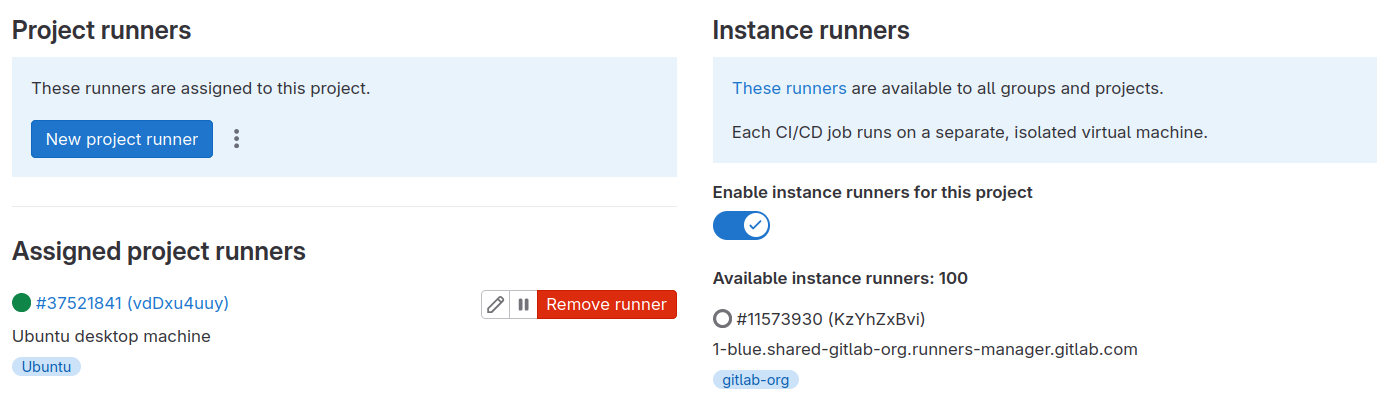
\includegraphics[width=5cm]{image/gitlab-runners.png} \\ Une machine match avec le tag \lstinline{Ubuntu} \\
        \end{columns}
    \end{frame}

    \begin{frame}
        \frametitle{GitLab}
        \framesubtitle{Exécution d'un pipeline sur un runner donné}
        \transdissolve
        La liste des exécutions des pipelines est dans Build > Pipelines~:
        \bigbreak
        \centering
        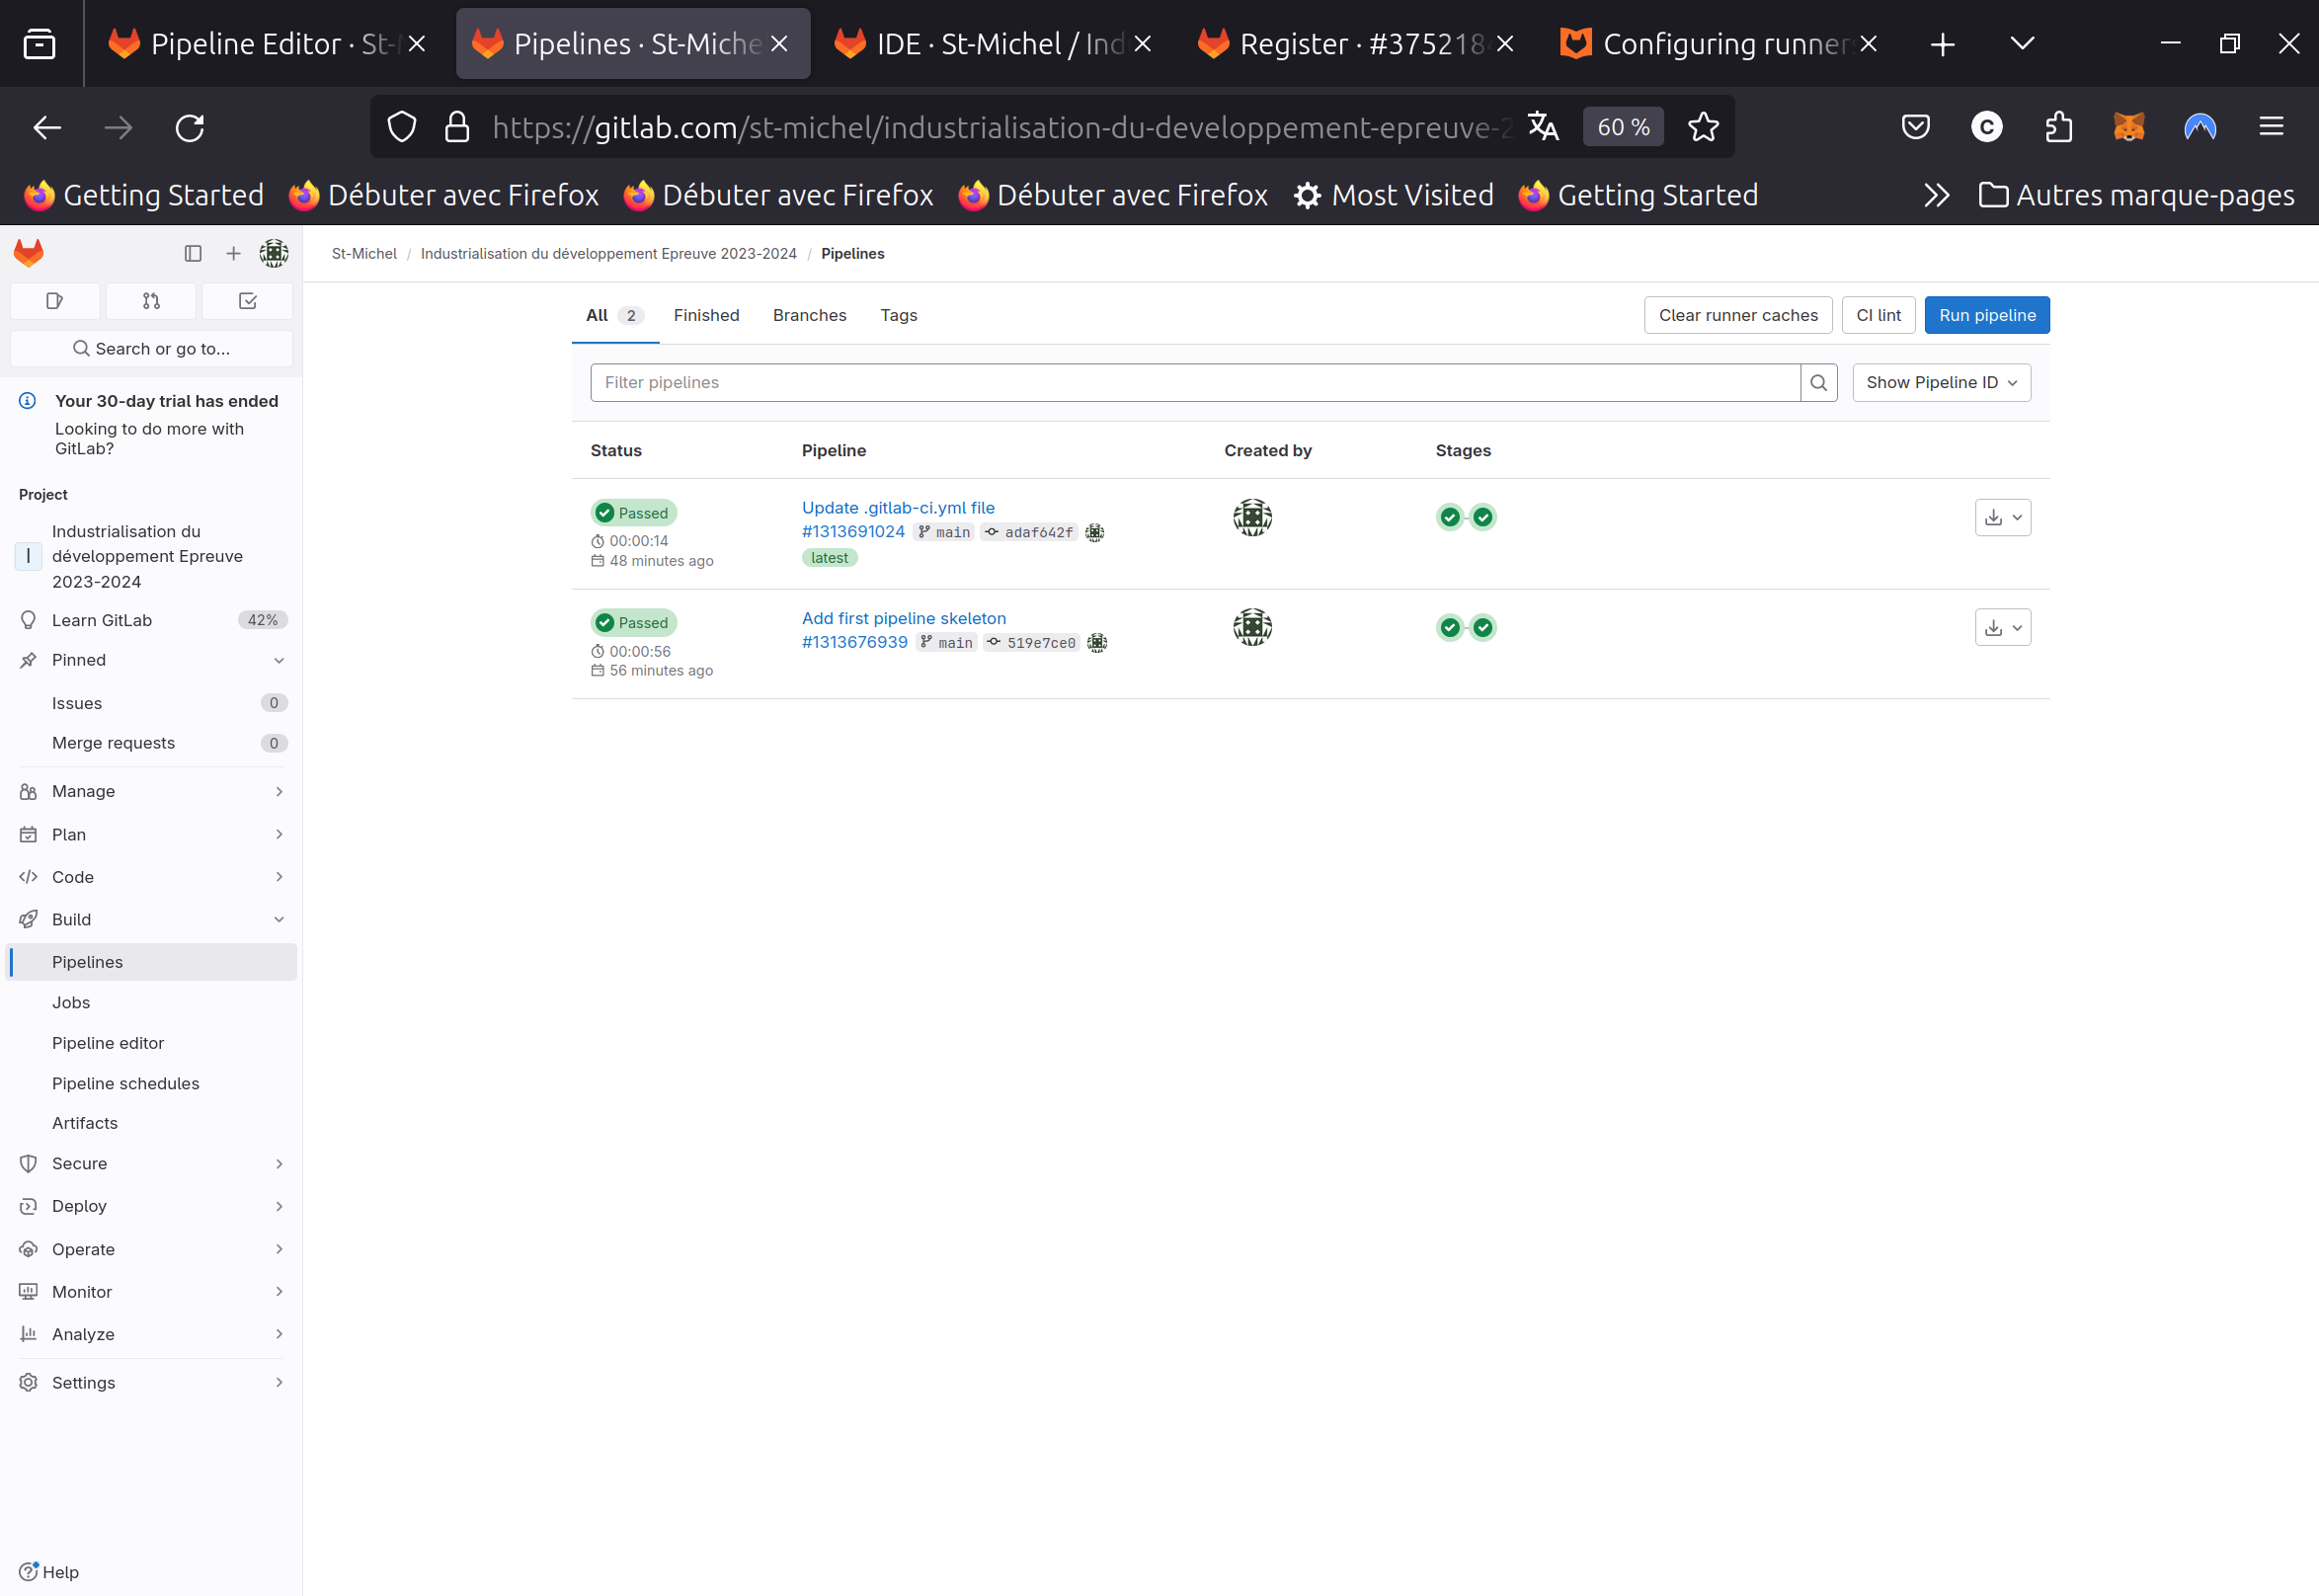
\includegraphics[width=10cm]{image/gitlab-pipelines-executions}
    \end{frame}

    \begin{frame}
        \frametitle{GitLab}
        \framesubtitle{Exécution d'un pipeline sur un runner donné}
        \transdissolve
        Il y a aussi une vue qui liste les Jobs est dans Build > Jobs~:
        \bigbreak
        \centering
        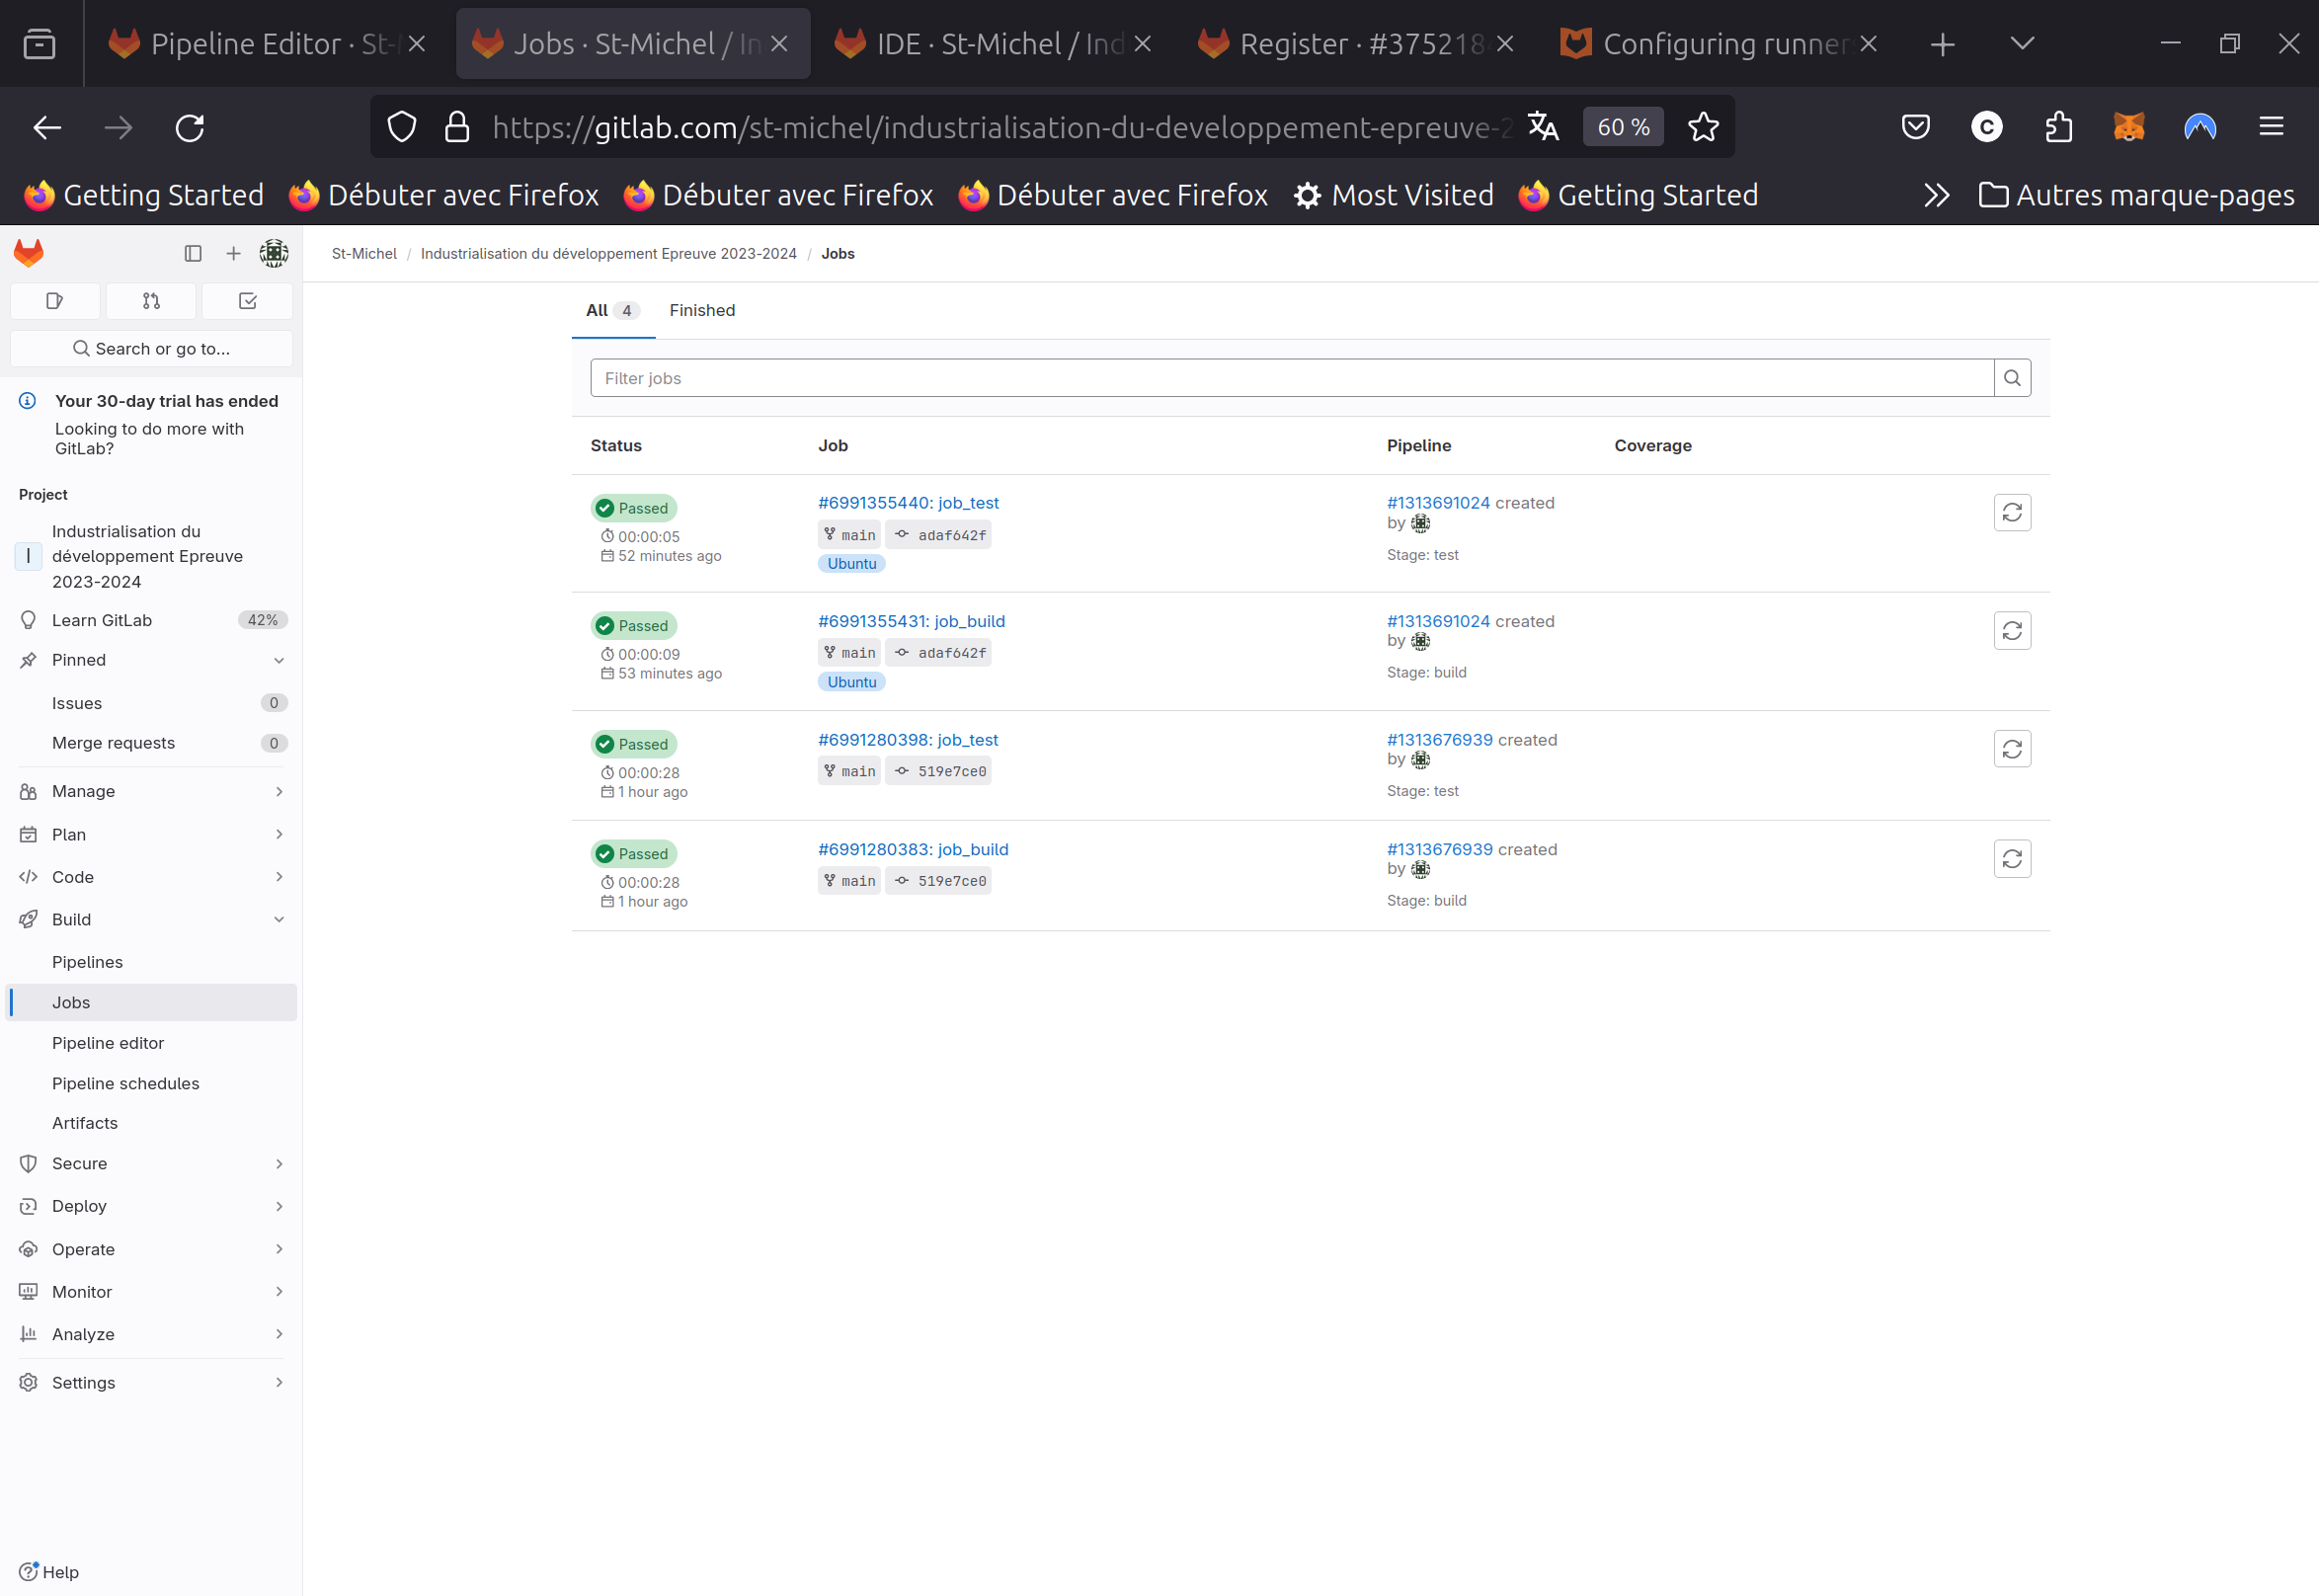
\includegraphics[width=10cm]{image/gitlab-jobs-executions}
    \end{frame}

    \begin{frame}
        \frametitle{GitLab}
        \framesubtitle{Exécution d'un pipeline sur un runner donné}
        \transdissolve
        Une vue détaillée des Jobs d'un Pipeline donné dans Build > Pipelines~:
        \bigbreak
        \centering
        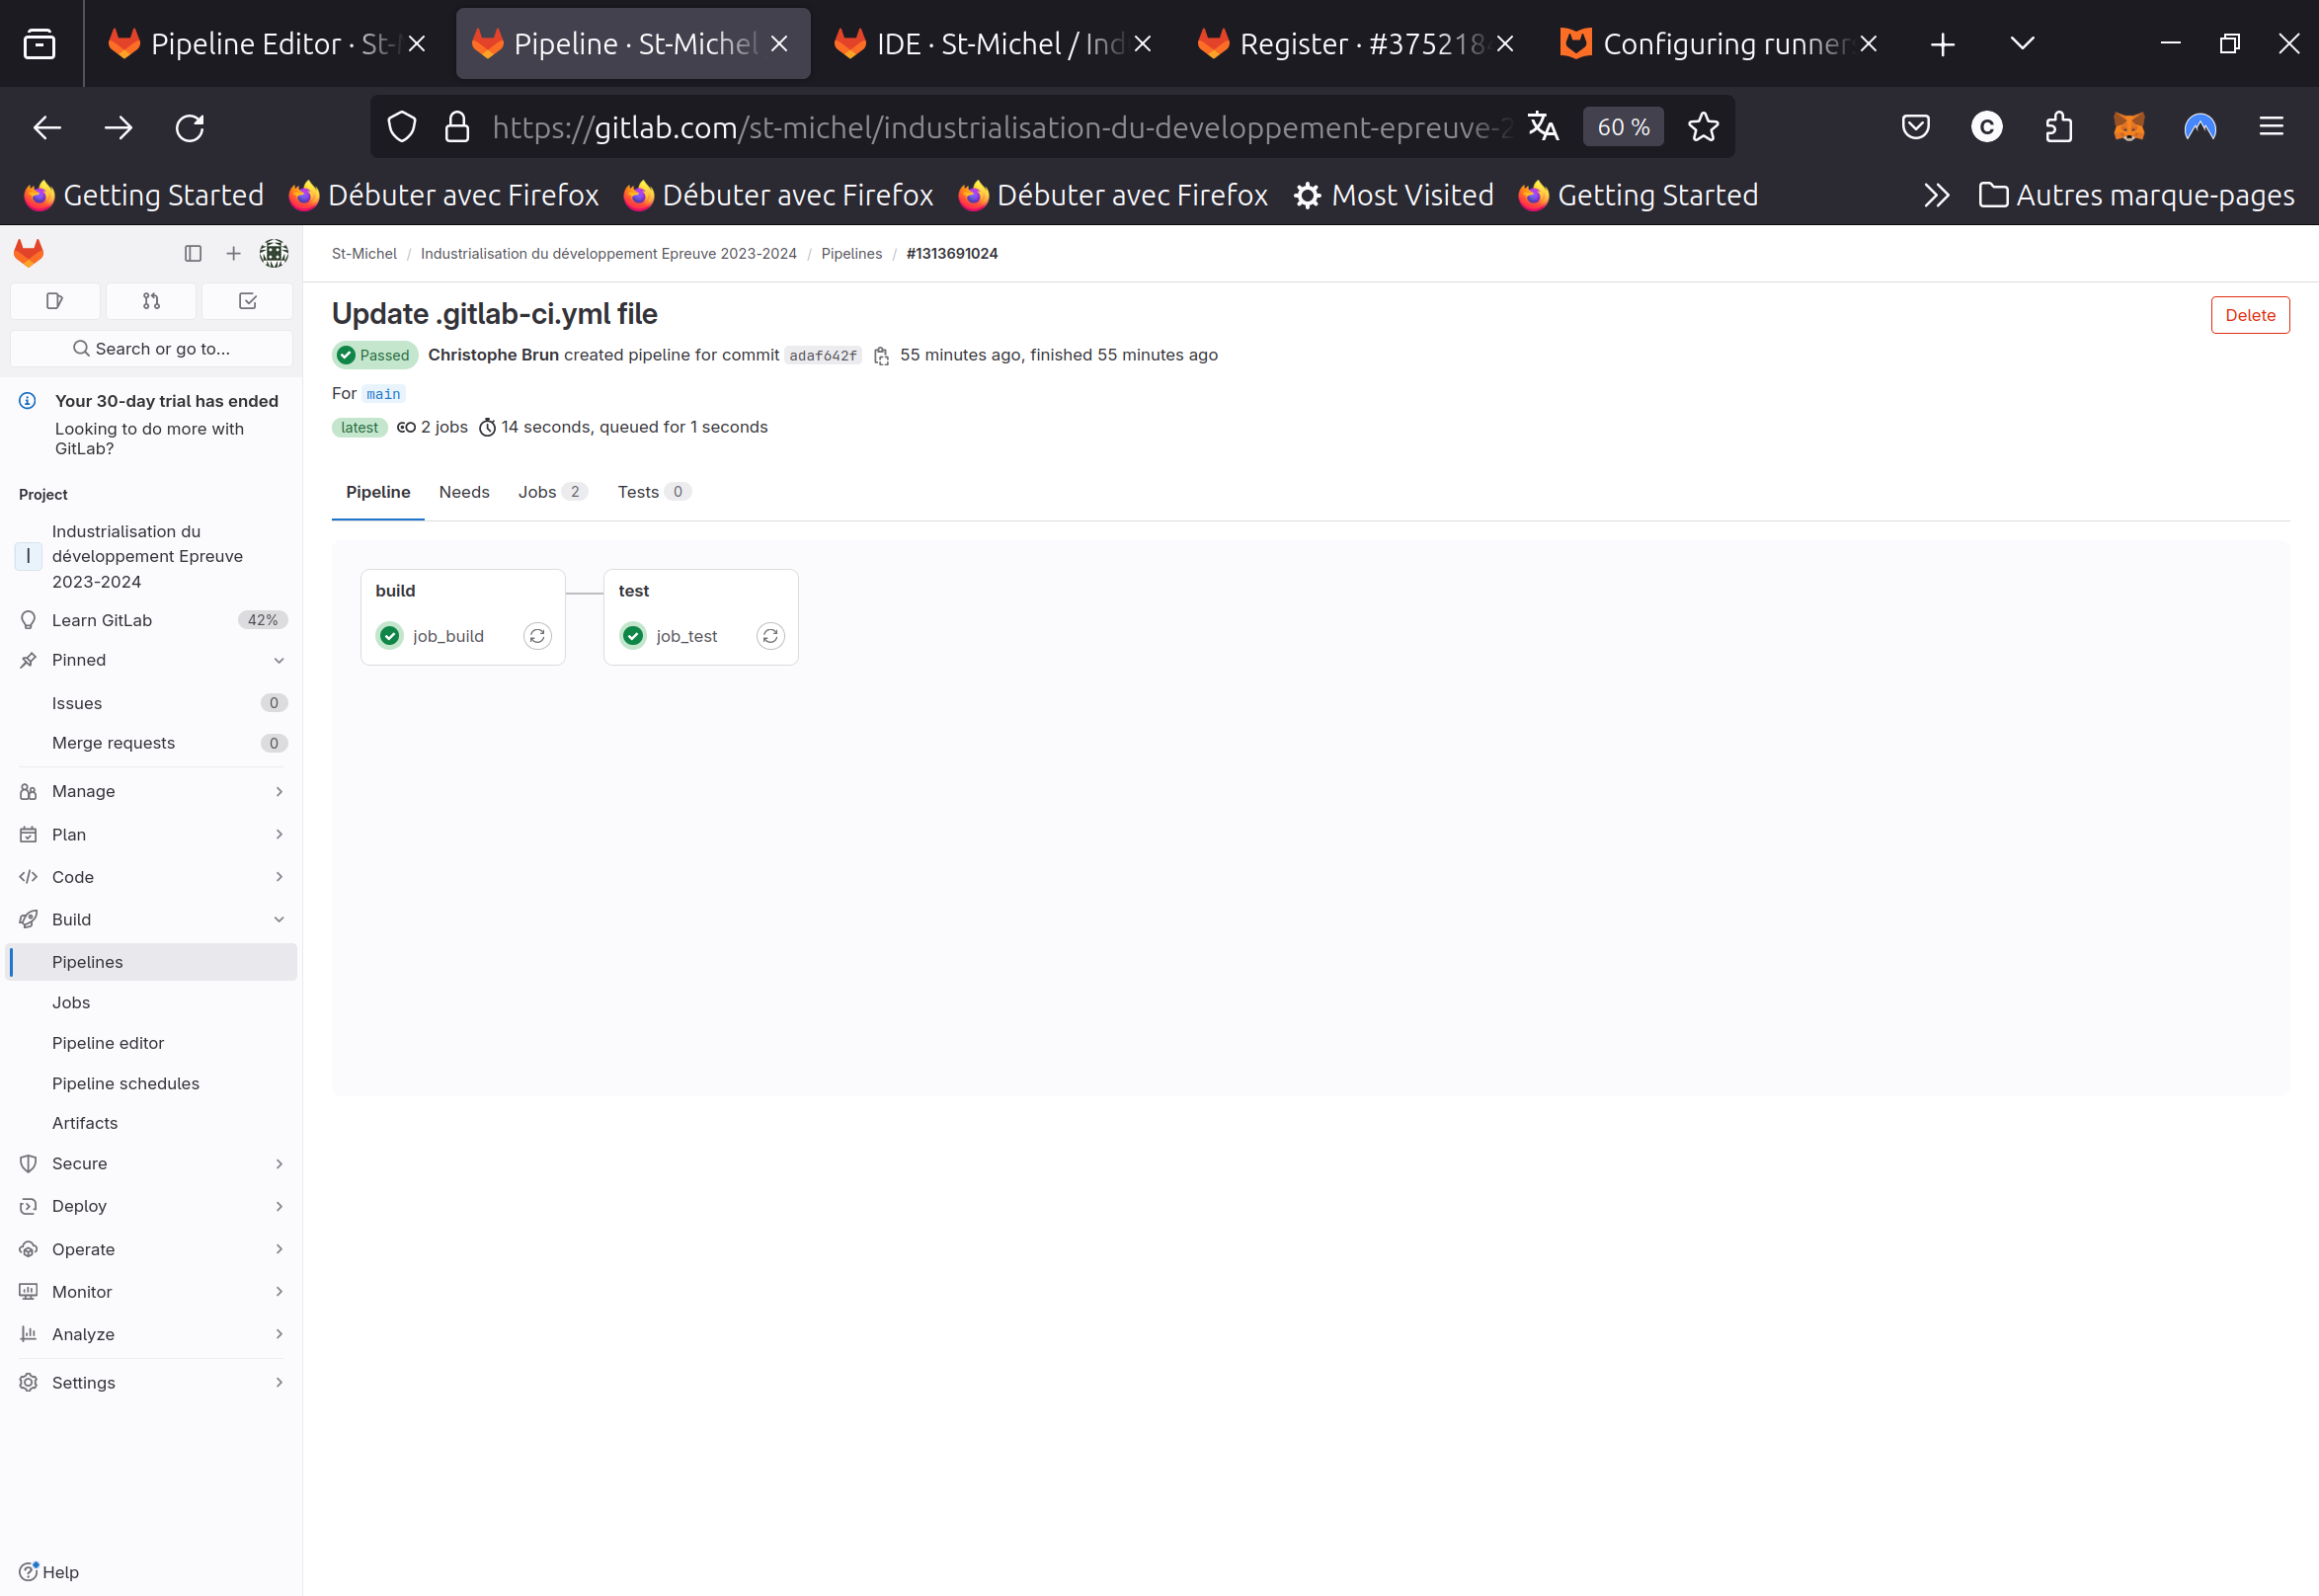
\includegraphics[width=10cm]{image/gitlab-pipeline-jobs-executions}
    \end{frame}

    \begin{frame}
        \frametitle{GitLab}
        \framesubtitle{Exécution d'un pipeline sur un runner donné}
        \transdissolve
        Une vue détaillée d'un Job avec les logs horodatées du runner~:
        \bigbreak
        \centering
        \includegraphics[width=10cm]{image/gitlab-pipeline-job-details}
    \end{frame}

    \subsection{Conclusion}\label{subsec:conclusion}
    \begin{frame}
        \frametitle{Risques cyber lié au CI/CD}
        \framesubtitle{Quels sont les risques cyber lié au CI/CD~?}
        \transdissolve
        \pause
        Une mauvaise configuration des droits, une faille non patchée, un secret exposé peuvent permettre d'accéder au données du CI/CD~.
        Donc probablement le code source.

        Exemples de hacks majeurs liés au CI/CD~:
        \begin{itemize}
            \item TeamCity non patché dans l'attaque de SolwarWinds\footnote{Echoes of SolarWinds, \url{https://www.scmagazine.com/news/echoes-of-solarwinds-jetbrains-teamcity-servers-under-attack-by-russia-backed-hackers}}.
            Un fournisseur de services et logiciels de supervision de réseau.
            Les hackers ont ensuite exploité les failles de Solar Winds et accédé aux réseaux des clients comme MS qui a vu un source de Windows fuiter.
            \item Circle CI a vu des secrets exposés\footnote{The CircleCI secrets hack is a red flag for security teams on software supply chain risk, \url{https://www.reversinglabs.com/blog/circleci-hack-is-a-red-flag-for-security-teams-on-the-software-supply-chain}}.
            Le hack n'a pas touché ceux qui avait mis en place Open ID Connect, la configuration est donc importante.
        \end{itemize}
    \end{frame}

    \begin{frame}
        \frametitle{Conclusions sur le CI/CD}
        \transdissolve
        \begin{itemize}
            \item C'est un outil de plus pour améliorer la qualité des livrables (documentation, rapport de tests, librairies, exécutables, etc).
            \item Pour éliminer du bug.
            \item Un outil collaboratif pour partager les résultats dans l'équipe et l'entreprise.
            \item Faire d'abord en local puis exécuter dans la plateforme CI/CD~.
            \item S'inspirer des outils qu'on a vue dans ou l'IDE ou en testing pour écrire des scripts.
            \item Attention aux ressources sur les machines locales.
            \item Attention aux coûts sur le cloud.
        \end{itemize}
    \end{frame}
\end{document}
